\documentclass[a4paper,12pt,oneside]{book} % nie: report!


% pakiety
\usepackage{polski} % lepiej to zamiast babel!
\usepackage[utf8]{inputenc} % w razie kłopotów spróbować: \usepackage[utf8x]{inputenc}
\usepackage{fancyhdr} % nagłówki i stopki
\usepackage{indentfirst} % WAŻNE, MA BYĆ!
\usepackage{lipsum}
\usepackage[pdftex]{graphicx} % to do wstawiania rysunków
\usepackage{amsmath} % to do dodatkowych symboli, przydatne
\usepackage[pdftex,
            left=1in,right=1in,
            top=1in,bottom=1in]{geometry} % marginsy
\usepackage{amssymb} % to też do dodatkowych symboli, też przydatne
\usepackage{pdfpages} % żeby wstawić stronę tytułową
% jesli potrzeb, można oczywiście wstawić inne pakiety i swoje definicje...
\usepackage{graphicx}
\graphicspath{{./pictures}}
\usepackage{import}

\usepackage{pgfplots}

\usepackage{xstring}
\usepackage{tikz}
\usepackage{listofitems}
\usepackage{etoolbox}
\usepackage{listings}
\usetikzlibrary{arrows.meta, fit, positioning} % for arrow size
\usepackage[outline]{contour} % glow around text
\contourlength{1.4pt}
\tikzstyle{mynode}=[thick,draw=blue,fill=blue!20]
\usetikzlibrary{shapes, positioning}
\tikzset{>=latex} % for LaTeX arrow head
\usepackage{xcolor}
\colorlet{myred}{red!80!black}
\colorlet{myblue}{blue!80!black}
\colorlet{mygreen}{green!60!black}
\colorlet{myorange}{orange!70!red!60!black}
\colorlet{mydarkred}{red!30!black}
\colorlet{mydarkblue}{blue!40!black}
\colorlet{mydarkgreen}{green!30!black}
\tikzstyle{node}=[thick,circle,draw=myblue,minimum size=22,inner sep=0.5,outer sep=0.6]
\tikzstyle{node in}=[node,green!20!black,draw=mygreen!30!black,fill=mygreen!25]
\tikzstyle{node hidden}=[node,blue!20!black,draw=myblue!30!black,fill=myblue!20]
\tikzstyle{node out}=[node,red!20!black,draw=myred!30!black,fill=myred!20]
\tikzstyle{connect}=[thick,mydarkblue] %,line cap=round
\tikzstyle{connect arrow}=[-{Latex[length=4,width=3.5]},thick,mydarkblue,shorten <=0.5,shorten >=1]
\tikzset{ % node styles, numbered for easy mapping with \nstyle
	node 1/.style={node in},
	node 2/.style={node hidden},
	node 3/.style={node out},
}
\def\nstyle{int(\lay<\Nnodlen?min(2,\lay):3)} % map layer number onto 1, 2, or 3

% VAE
\newcommand\drawEncoder[2]{
	% #1 (str): namespace
	% #2 (list[list[str]]): list of labels to print in the node of each neuron
	\foreach \neurons [count=\lyrIdx] in #2 {
		\ifnum \lyrIdx = 1
			\StrCount{\neurons}{,}[\lyrLength]
			\foreach \n [count=\nIdx] in \neurons
			\node[myin] (#1-\lyrIdx-\nIdx) at (2*\lyrIdx, \lyrLength/2-1.4*\nIdx) {$x_\nIdx$};
		\else 
			\StrCount{\neurons}{,}[\lyrLength] 
			\foreach \n [count=\nIdx] in \neurons
			\node[hidden] (#1-\lyrIdx-\nIdx) at (2*\lyrIdx, \lyrLength/2-1.4*\nIdx) {\n};
		\fi
	}
}

\newcommand\drawDecoder[2]{
	% #1 (str): namespace
	% #2 (list[list[str]]): list of labels to print in the node of each neuron
	\foreach \neurons [count=\lyrIdx] in #2 {
		\ifnum \lyrIdx = 3
			\StrCount{\neurons}{,}[\lyrLength]
			\foreach \n [count=\nIdx] in \neurons
			\node[myout] (#1-\lyrIdx-\nIdx) at (2*\lyrIdx, \lyrLength/2-1.4*\nIdx) {$\hat{x}_\nIdx$};
		\else 
			\StrCount{\neurons}{,}[\lyrLength] 
			\foreach \n [count=\nIdx] in \neurons
			\node[hidden] (#1-\lyrIdx-\nIdx) at (2*\lyrIdx, \lyrLength/2-1.4*\nIdx) {\n};
		\fi
	}
}
\newcommand\denselyConnectNodes[2]{
	% #1 (str): namespace
	% #2 (list[int]): number of nodes in each layer
	\foreach \n [count=\lyrIdx, remember=\lyrIdx as \previdx, remember=\n as \prevn] in #2 {
		\foreach \y in {1,...,\n} {
			\ifnum \lyrIdx > 1
			\foreach \x in {1,...,\prevn}
			\draw[connect] (#1-\previdx-\x) -- (#1-\lyrIdx-\y);
			\fi
		}
	}
}


% definicje nagłówków i stopek
\pagestyle{fancy}
\renewcommand{\chaptermark}[1]{\markboth{#1}{}}
\renewcommand{\sectionmark}[1]{\markright{\thesection\ #1}}
\fancyhf{}
\fancyhead[LE,RO]{\footnotesize\bfseries\thepage}
\fancyhead[LO]{\footnotesize\rightmark}
\fancyhead[RE]{\footnotesize\leftmark}
\renewcommand{\headrulewidth}{0.5pt}
\renewcommand{\footrulewidth}{0pt}
\addtolength{\headheight}{1.5pt}
\fancypagestyle{plain}{\fancyhead{}\cfoot{\footnotesize\bfseries\thepage}\renewcommand{\headrulewidth}{0pt}}

% interlinia
\linespread{1.25}


% treść
\begin{document}
\sloppy

\thispagestyle{empty}

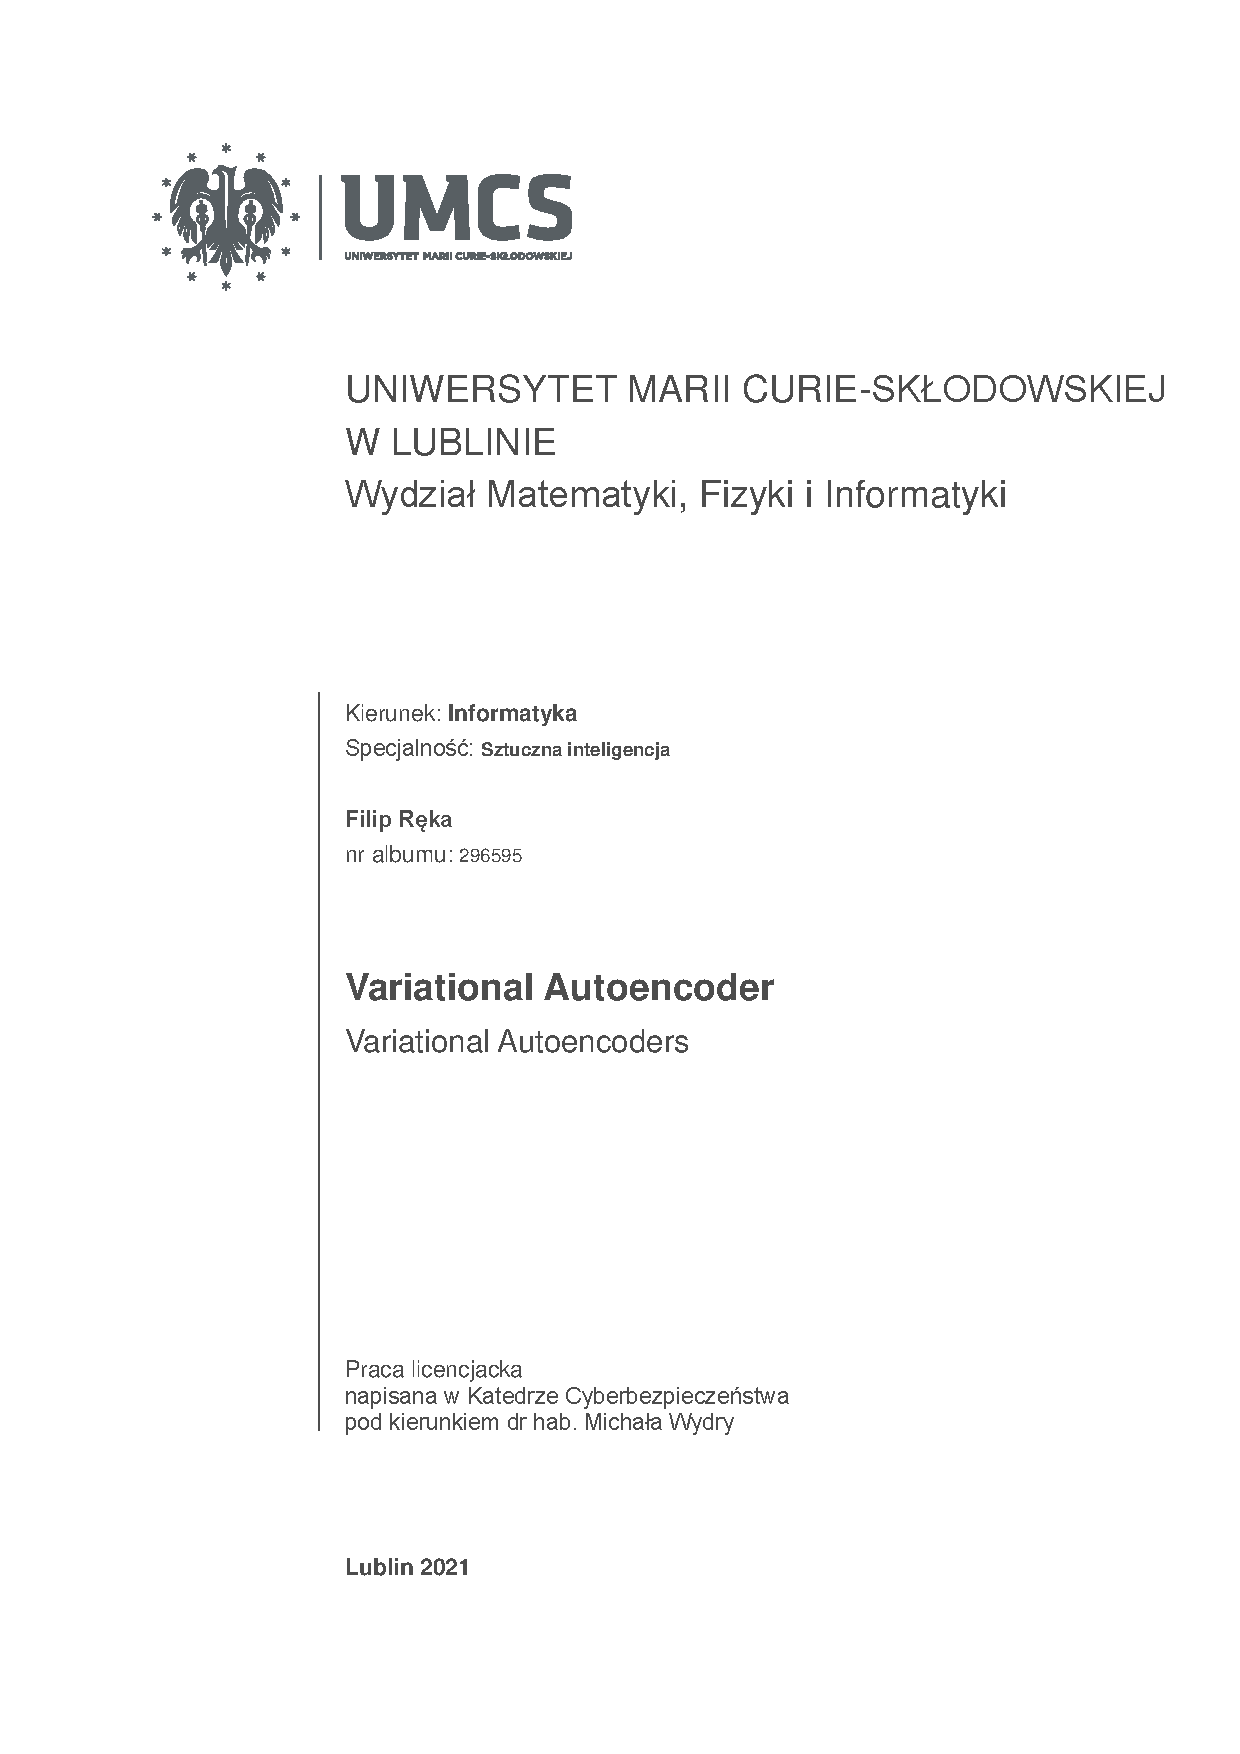
\includepdf{stronatytulowasvg}

\tableofcontents{}

\chapter*{Wstęp} % z gwiazdką, więc bez numerka...
\addcontentsline{toc}{chapter}{Wstęp} % ...ale w spisie treści ma być
\textbf{Autoenkoder} jest jednym z rodzajów sieci neuronowych, której zadaniem jest nauczenie się zakodowania nieoznaczonych danych. Kod jest wykorzystywany do ponownego, jak najlepszego, wygenerowania wejścia sieci. Autoenkoder uczy się reprezentacji zbioru danych jako zmiennych ukrytych przez ignorowanie nieistotnych części danych.
Wariacyjne autoenkodery są popularnymi modelami generacyjnymi. Zostały zaproponowane przez Diederika P. Kingma i Maxa Wellinga w roku 2014 \cite{kingma2014autoencoding}. Najczęściej zostają one skategoryzowane do modeli uczenia częściowo nadzorowanego. Znajdują zastosowanie w generacji obrazów, tekstu, muzyki oraz w detekcji anomalii. W przeciwieństwie do tradycyjnych autoenkoderów prezentują pobabilistyczne podejście do generowania zmiennych ukrytych. Swoją popularność zawdzięcza swojej budowie, która jest oparta na sieciach neuronowych oraz możliwości trenowania ich przy pomocy metod gradientowych.
\chapter{Tradycyjny autoenkoder} 
\section{Informacje wstępne}
Autoenkoder (AE) jest specyficzną wersją sieci neuronowej składającej się z dwóch części: enkodera, który koduje dane wejściowe oraz dekodera, który na podstawie kodu rekonstruuje wejście \cite{bank2021autoencoders}. Architektura enkodera wymaga, aby jego warstwa wyjściowa generująca reprezentacje danych była mniejsza niż warstwa wejściowa. Często zwężenie to jest nazywane \textit{bottle neck}. Model na swoją warstwę wejściową oraz wyjściową dostaje te same dane. Powiedzmy że mamy dane wejściowe $X$ o wymiarze $m$ oraz chcemy je zakodować do wymiaru $n$. Formalnie możemy zapisać:\\
\begin{center}
	Enkoder $E: \mathbb{R}^m \rightarrow \mathbb{R}^n$\\
	Dekoder $D: \mathbb{R}^n \rightarrow \mathbb{R}^m$ \\
	gdzie $n < m$\\
\end{center}
Celem \textit{bottle neck-a} jest skompresowanie wejścia i zachowanie w ukrytych wartościach jak najwięcej informacji. W momencie, kiedy $n = m$, model przekazałby wartości z pierwszej warstwy na ostatnią bez potrzeby kompresji. Celem treningu całego autoenkodera jest zminimalizowanie błędu pomiędzy prawdziwymi danymi wejściowymi a tymi odkodowanymi ze skompresowanych wartości. W przypadku obrazów funkcją straty może być na przykład błąd średniokwadratowy lub binarna entropia krzyżowa, która powie nam, jak wynik różni się od wejścia. 
 \begin{center}
 		$\mathcal{L}(x, \hat{x}) = \dfrac{1}{m}\displaystyle\sum_{i=0}^{m}(x_i-\hat{x}_i)^2 = \dfrac{1}{m}\displaystyle\sum_{i=0}^{m}(x_i-D(E(x_i)))^2$
 \end{center}

%\begin{figure}[h]
%	\centering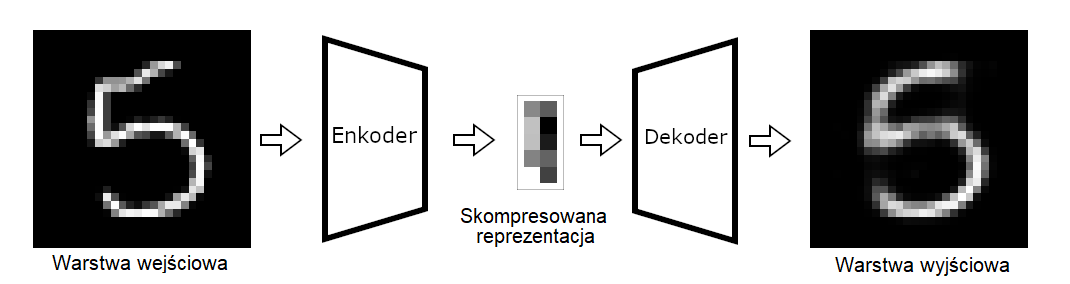
\includegraphics[width=14.5cm]{autoencoder.png}
%	\caption{Schemat budowy autoenkodera.}
%\end{figure}
\begin{figure}[h!]
	\centering
	\begin{tikzpicture}
		\node (true) at (-6, 0) {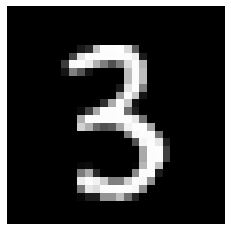
\includegraphics[width=3.5cm]{aeorg.png}};
		\draw[thick] (-3.4, 1.5) -- (-3.4, -1.5) node[pos=0.5] (enkoderin){} -- (-1.7, -0.8) -- (-1.7, 0.8) node[pos=0.5] (enkoderout){} -- cycle;
		\draw[-latex, thick] (true.east) -- (enkoderin.west);    
				\node[scale=0.7] (sample) at (0, 0) {\(\begin{bmatrix}
				3.18 \\ 1.83 \\ \vdots \\ 0.71 \\ 2.94
			\end{bmatrix}\)};                                     
		\draw[-latex, thick](enkoderout.east) -- (sample.west);                                                                                 
		\draw[thick] (1.7, 0.8) -- (1.7, -0.8) node[pos=0.5] (dekoderin){} -- (3.4, -1.7) -- (3.4, 1.7) node[pos=0.5] (dekoderout){} -- cycle;
		\node (recon) at (6, 0) {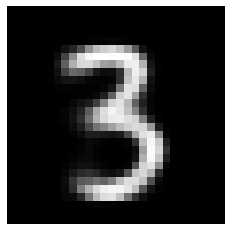
\includegraphics[width=3.5cm]{aerec.png}};
		\draw[-latex, thick](sample.east) -- (dekoderin.west);
		\draw[-latex, thick](dekoderout.east) -- (recon.west);
		% Labels
		\node at (-6, -2.2) {wejście};
		\node at (6, -2.2) {wyjście};
		\node at (0, -1.5) {wektor kodu};
		\node at (-2.52, 0) {enkoder};
		\node at (2.52, 0) {dekoder};
		
	\end{tikzpicture}
	\caption{Schemat budowy autoenkodera.}
	\label{fig:aeschemat}
\end{figure}
\newpage
\subsection{Zbiór danych MNIST}
Zbiór danych MNIST (\textit{Modified National Institute of Standards and Technology}) jest zbiorem wielu odręcznie pisanych cyfr \cite{mnist}. Znajduje szerokie zastosowanie w nauce i prezentacjach możliwości modeli uczenia maszynowego. W jego skład wchodzi 60 000 obrazów przeznaczonych do treningu modeli oraz 10 000 do testów. Obrazy są czarno-białe i mają wymiary 28 na 28 pikseli.
\begin{figure}[h]
	\centering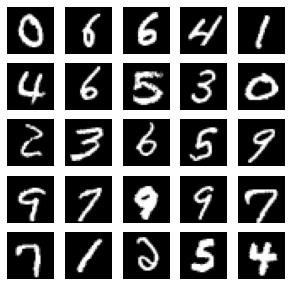
\includegraphics[width=5cm]{pictures/mnist.png}
	\caption{Przykładowe obrazy ze zbioru danych.}
\end{figure}
\newpage
\section{Budowa}
W skład autoenkodera wchodzi enkoder oraz dekoder. Obie części są w pełni połączonymi sieciami neuronowymi, połączonymi również pomiędzy sobą. Prosta budowa sprawia, że bez problemu obie sieci są trenowane równocześnie.
\begin{figure}[!h]
\centering
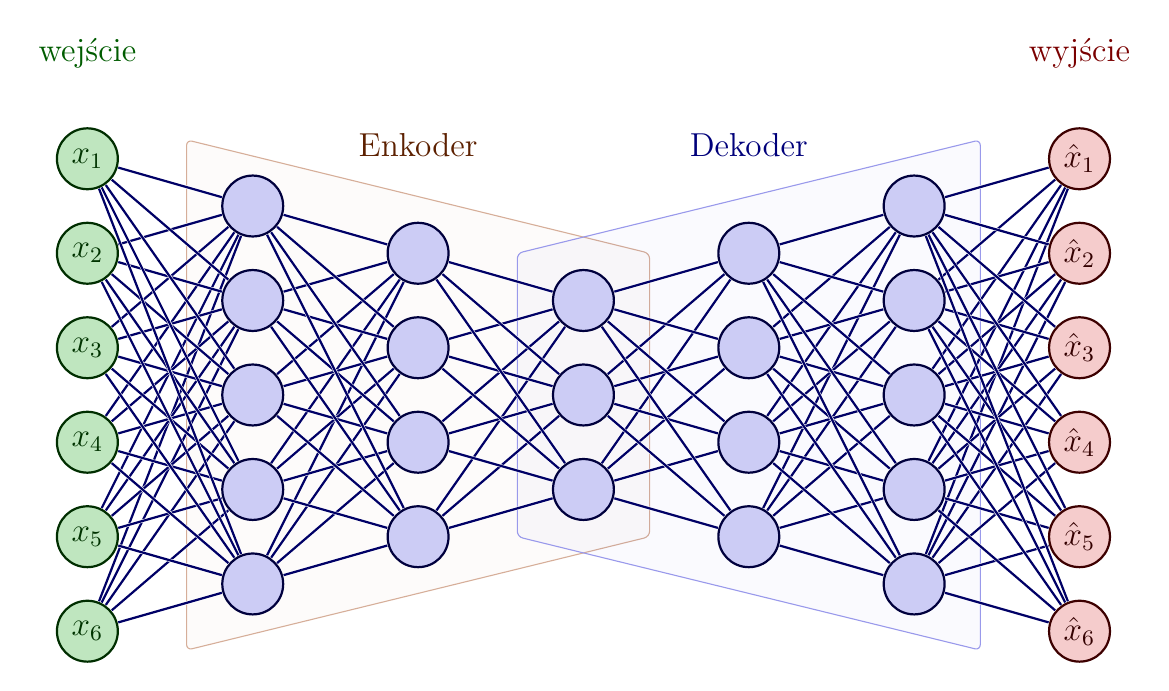
\begin{tikzpicture}[x=2.1cm,y=1.2cm]
	\large
	\readlist\Nnod{6,5,4,3,4,5,6} % array of number of nodes per layer
	
	% TRAPEZIA
	\node[above,align=center,myorange!60!black] at (3,2.4) {Enkoder};
	\node[above,align=center,myblue!60!black] at (5,2.4) {Dekoder};
  	\draw[myorange!40,fill=myorange,fill opacity=0.02,rounded corners=2]
		(1.6,-2.7) --++ (0,5.4) --++ (2.8,-1.2) --++ (0,-3) -- cycle;
	\draw[myblue!40,fill=myblue,fill opacity=0.02,rounded corners=2]
		(6.4,-2.7) --++ (0,5.4) --++ (-2.8,-1.2) --++ (0,-3) -- cycle;
	
	\foreachitem \N \in \Nnod{ % loop over layers
		\def\lay{\Ncnt} % alias of index of current layer
		\pgfmathsetmacro\prev{int(\Ncnt-1)} % number of previous layer
		\message{\lay,}
		\foreach \i [evaluate={\y=\N/2-\i+0.5; \x=\lay; \n=\nstyle;}] in {1,...,\N}{ % loop over nodes
			
			% NODES
			\ifnum \Ncnt = 1
				\node[node \n,outer sep=0.6] (N\lay-\i) at (\x,\y) {$x_\i$};
			\else
				\ifnum \Ncnt = 7
					\node[node \n,outer sep=0.6] (N\lay-\i) at (\x,\y) {$\hat{x}_\i$};
				\else
					\node[node \n,outer sep=0.6] (N\lay-\i) at (\x,\y) {};
				\fi
			\fi
			
			% CONNECTIONS
			\ifnumcomp{\lay}{>}{1}{ % connect to previous layer
				\foreach \j in {1,...,\Nnod[\prev]}{ % loop over nodes in previous layer
					\draw[connect,white,line width=1.2] (N\prev-\j) -- (N\lay-\i);
					\draw[connect] (N\prev-\j) -- (N\lay-\i);
					%\draw[connect] (N\prev-\j.0) -- (N\lay-\i.180); % connect to left
				}
			}{} % else: nothing to connect first layer
			
		}
	}
	
	% LABELS
	\node[above=0.5,align=center,mygreen!60!black] at (N1-1.90) {wejście};
	\node[above=0.5,align=center,myred!60!black] at (N\Nnodlen-1.90) {wyjście};
	
\end{tikzpicture}
\caption{Wizualizacja sieci tworzącej autoenkoder.}
\label{fig:aenetwork}
\end{figure}\\
Obrazek \ref{fig:aenetwork} przedstawia prosty autoenkoder kompresujący sześciowymiarowe wejście do kodu o długości trzy. Enkoder, jak i dekoder mają dwie warstwy ukryte. Odbicie lustrzane architektury nie jest konieczne, aby model działał poprawnie, jednak zwyczajem jest używanie takiej architektury.\\
Hiperparametramy modelu, które możemy ustalić przed jego treningiem to:
\begin{itemize}
	\item Ilość warstw ukrytych - jeśli wiemy, że nasze dane są skomplikowane, dodatkowe warstwy ukryte będą miały pozytywny wpływ na otrzymywane rezultaty, ponieważ większa ilość warstw sprawia, że model jest w stanie nauczyć się bardziej skomplikowanych funkcji \cite{telgarsky2016benefits, eldan2016power}.
	\item Ilość neuronów w poszczególnych warstwach - autoenkoder powinien posiadać w każdej warstwie mniej neuronów niż w poprzedniej. W ten sposób model nie będzie ``oszukiwał" i zostaje zmuszony do reprezentacji jak najlepszej kompresji.
	\item Funkcja straty - najlepszymi funkcjami straty do treningu autoenkodera jest błąd średniokwadratowy lub binarna entropia krzyżowa w przypadku, kiedy dane są w przedziale od 0 do 1.
	\item Rozmiar kodu - jest to najistotniejszy parametr dla nas i dla modelu. Dłuższy kod oznacza zachowanie więcej istotnych elementów, a co za tym idzie lepsze odwzorowanie przez dekoder. Z drugiej strony, używając dłuższego wektora zmiennych ukrytych, dostajemy gorszą kompresje danych. Długość kodu musimy dobrać w zależności od problemu, który chcemy rozwiązać, używając model.
\end{itemize}
\section{Zastosowania}
\subsection{Redukcja wymiaru}
Żyjemy w świecie, który otacza nas coraz większą ilością informacji. Jej ilość sprawia, że możemy z niej wyciągać coraz to więcej ilości danych. Wiele z tych danych, takie jak obrazy, tekst czy nagrania są opisywane przez wiele parametrów. Redukcja wymiaru jest procesem zmniejszenia liczby zmiennych przeznaczonych do analizy, a zarazem zachowanie w nich jak najwięcej istotnych informacji. Powody, dla których chcemy zmniejszyć wymiarowość danych to między innymi:
\begin{itemize}
	\item Część zmiennych opisująca dane jest ze sobą nadmiernie skorelowana lub niesie ze sobą cechy, które nie są istotne statystycznie i usunięcie ich nie wpływa na poprawę działania modeli oraz czas ich treningu.
	\item Dane bardzo wysokiego wymiaru są trudne do analizy lub operacje na nich zajmują tak dużo czasu i zasobów, co sprawia, że stają się one bezużyteczne. 
	\item Wielowymiarowe dane jest ciężej zwizualizować. Możemy je zredukować do jedno-, dwu- lub trzywymiarowej reprezentacji, co pozwoli nam na proste narysowanie wykresu, który będzie prosty do zrozumienia.
\end{itemize}
Autoenkoder nie jest jednym sposobem na redukcję wymiarów. Najbardziej rozpowszechnioną metodą jest \textit{PCA}. 
\subsubsection{Analiza składowych głównych}
Analiza składowych głównych (\textit{ang. Principal Components Analysis, \textbf{PCA}}) służy do wyznaczania jak najmniejszej ilości nowych zmiennych, mówiących jak najwięcej o zbiorze danych. Wielowymiarowe dane koncentrują się w pewnych podprzestrzeniach oryginalniej przestrzeni. Analiza PCA pozwala znaleźć te podprzestrzenie, które są wektorami pełniącymi rolę nowych osi, które lepiej opisują nasz zbiór danych \cite{redukcjawymiarow}. Używając tej metody ograniczamy się tylko do przekształceń liniowych. Ilość wektorów, względem których można zredukować dane, jest równa wymiarowi danych. Środkowy obrazek na rysunku \ref{fig:pca} przedstawia właśnie te wektory na przykładzie dwuwymiarowego zbioru punków. Linia, względem której spłaszczane są dane, jest tą, która minimalizuje odległość do niej od wszystkich punktów. Dolny wykres rysunku \ref{fig:pca} pokazuje już spłaszczone dane do jednego wymiaru. Nowe wektory są wybierane w taki sposób, aby wariancja rzutów poszczególnych obserwacji była jak największa, co gwarantuje nam odwzorowanie jak największej ilości danych. Każdy kolejny wektor zachowuję się w taki sam sposób oraz jest ortonormalny do poprzednich.
\begin{figure}[h!]
	\centering
	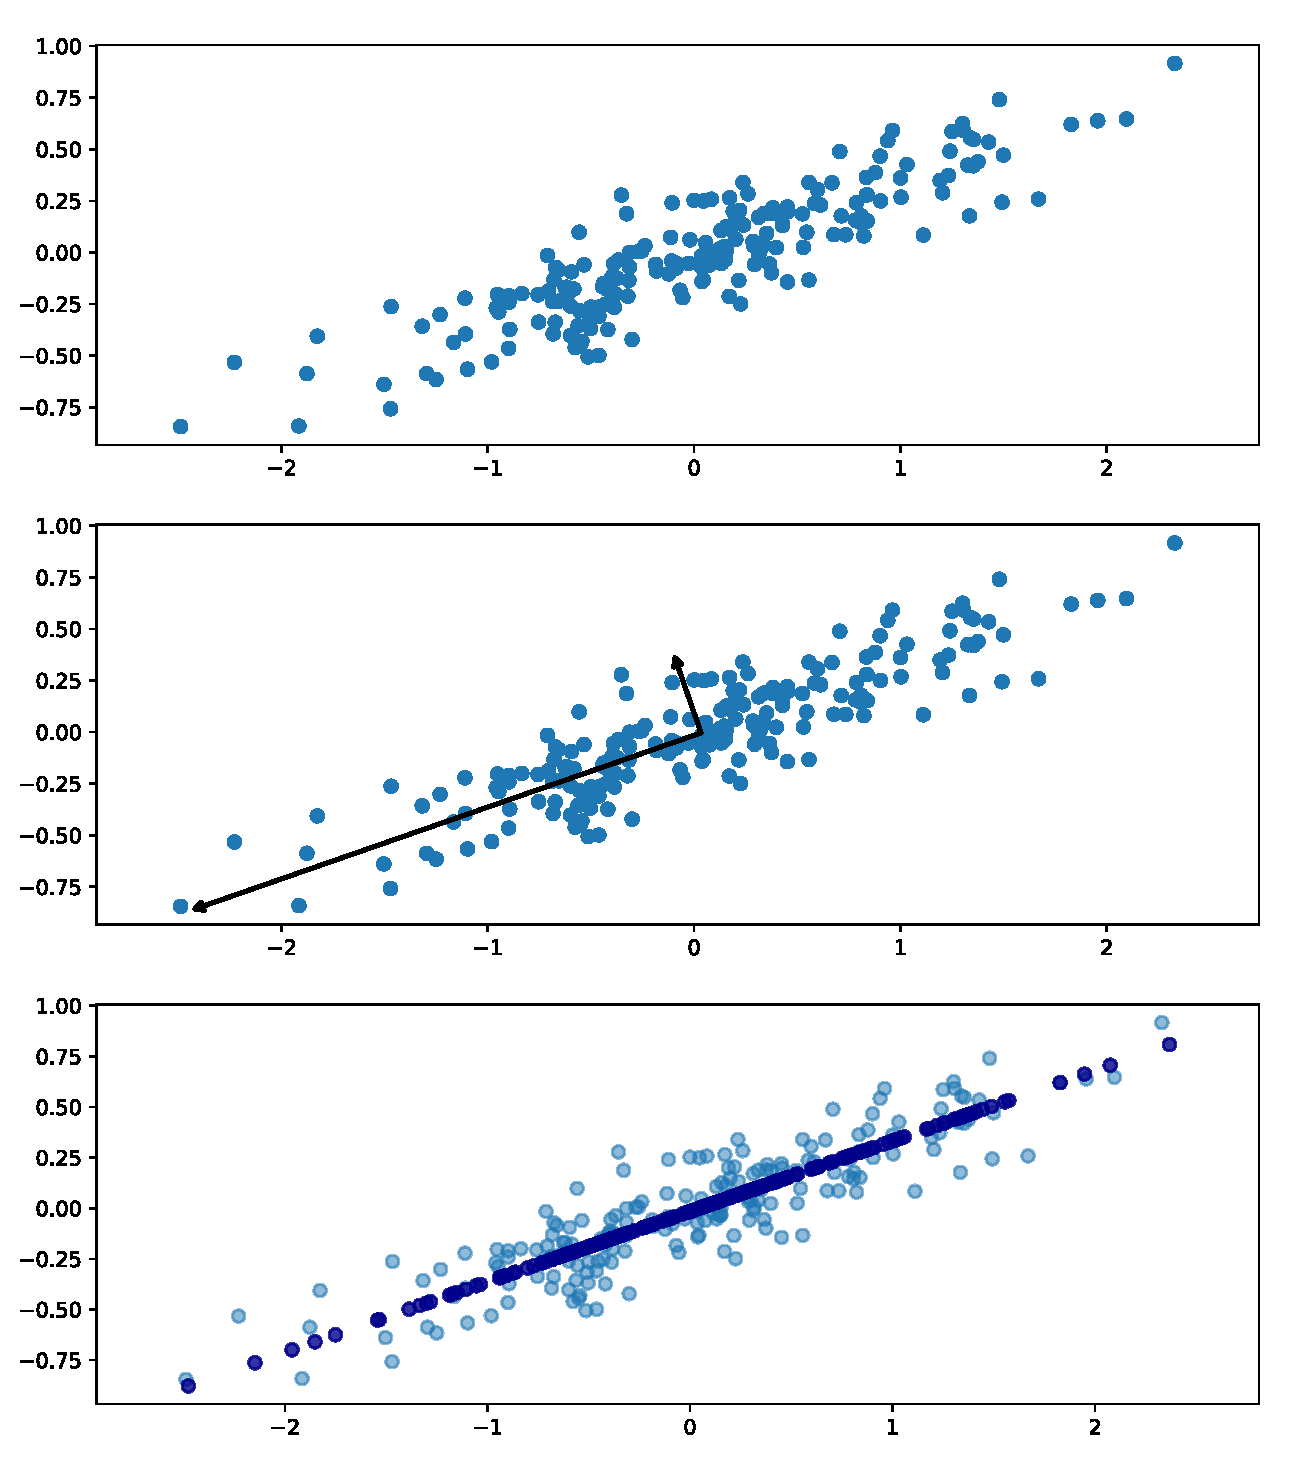
\includegraphics[width=\textwidth]{pca.pdf}
	\caption{Wizualizacja PCA na zbiorze punktów w przestrzeni dwuwymiarowej.}
	\label{fig:pca}
\end{figure}

Wykres \ref{fig:pcacumsum} pokazuje zależność między ilością składników PCA a procentem wariancji opisywanym przez składniki na podstawie zbioru danych MNIST. Ilość składników mieści się w przedziale od 1 do 784 (28 razy 28 pixeli). Jak można zauważyć, dane reprezentowane przez około 80 wartości są w stanie opisać 90\% wariancji danych, co jest znaczą redukcją z 784. Przy 400 składnikach osiągamy praktycznie 100\% pokrycia. 
\begin{figure}[h!]
	\centering
	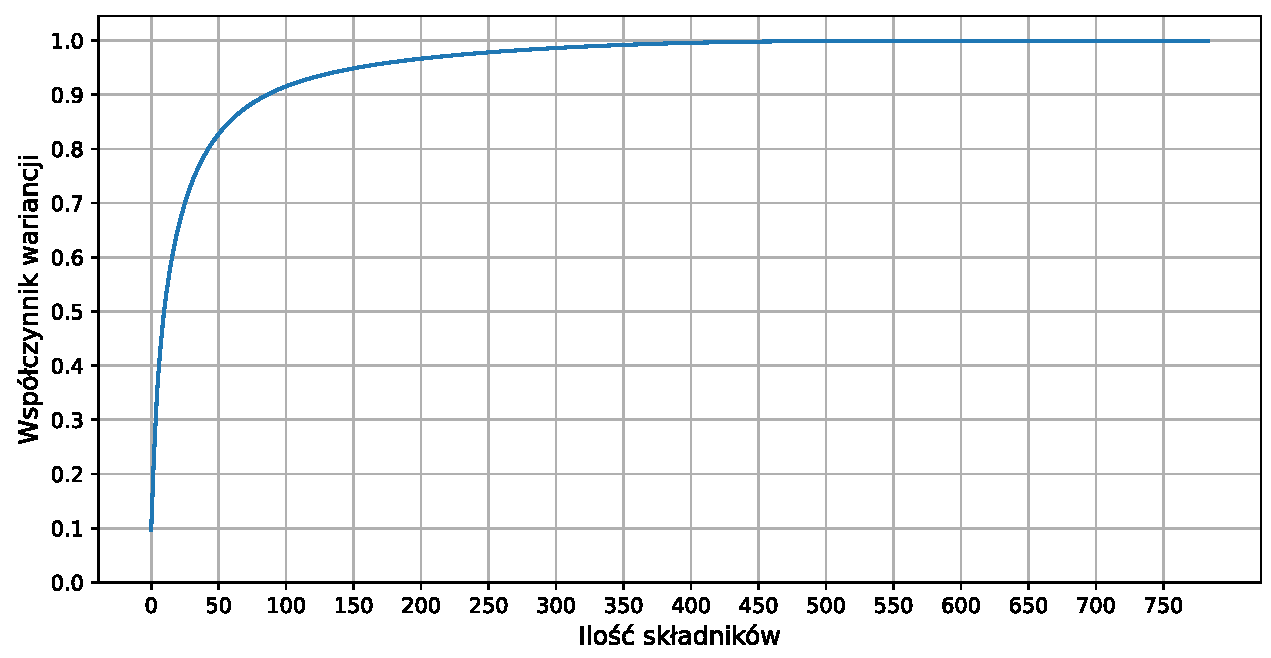
\includegraphics[width=\textwidth]{pcacumsum.pdf}
	\caption{Procent wariancji opisywany przez ilość składników.}
	\label{fig:pcacumsum}
\end{figure}
\subsubsection{Autoenkoder}
Użycie autoenkodera jest jedną z możliwości, jaką mamy, jeśli chcemy dokonać redukcji wymiarów. Jego budowa wymusza naukę jak najlepszej reprezentacji danych w kodzie. Zadaniem enkodera jest zachowanie w zmiennych jak najwięcej informacji dotyczących wejścia, a dekoder odwzorować jak najwięcej z nich. Najważniejszą cechą autoenkodera jest możliwość nauki przekształceń zarówno liniowych, jak i nieliniowych w zależności od doboru funkcji aktywacji.
\begin{figure}[h!]
	\centering
	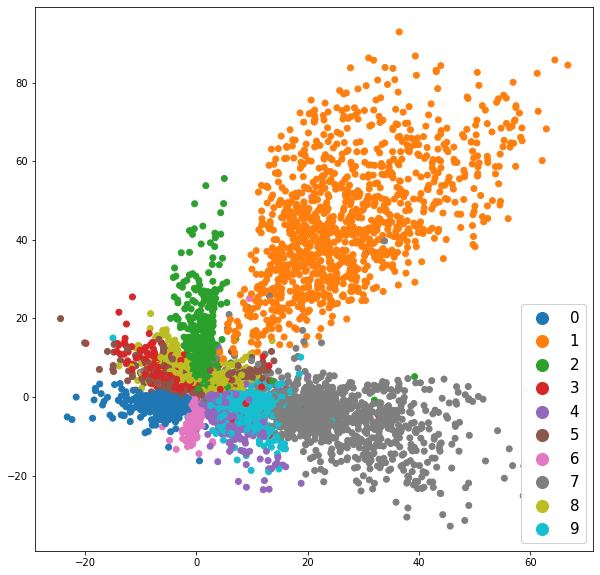
\includegraphics[width=10.5cm]{pictures/aelatentspace.png}
	\caption{Przestrzeń dwuwymiarowej zmiennej ukrytej dla zbioru MNIST.}
	\label{fig:latentspaceae}
\end{figure}

\subsubsection{Porównanie obu metod}
Obie przedstawione metody redukowania wymiarów są bardzo dobrymi wyborami. Wybór jednej z nich powinien zostać dopasowany do naszych potrzeb i do zbioru danych, którego używamy. PCA, będąc ograniczone do jedynie liniowych przekształceń, jest szybsze niż autoenkoder, który wymaga treningu. Jest ono też lepszym wyborem, kiedy wiemy, że nasze dane są nadmiernie skorelowane. Rozpatrzmy przykład zbioru danych opisującego takie cechy ludzi, jak wzrost, waga, kolor oczu oraz długość włosów. Wiemy, że czyjaś waga jest zależna od wzrostu. PCA w takim przykładzie bez problemu odnajdzie tą zależność i zredukuje. Autoenkoder jest lepszym wyborem, kiedy mamy do czynienia z danymi, które są o wiele bardziej złożone, czyli obrazy czy pliki audio. Różnica pomiędzy nauką liniowych oraz nielinowych przekształceń została pokazana na rysunku \ref{fig:pcavsautoenkoder}.  
Jednowarstwowy autoenkoder z liniową funkcją aktywacji na każdej warstwie zachowuje się dokładnie tak samo jak PCA \cite{aevspca}.
\begin{figure}[h!]
	\centering
	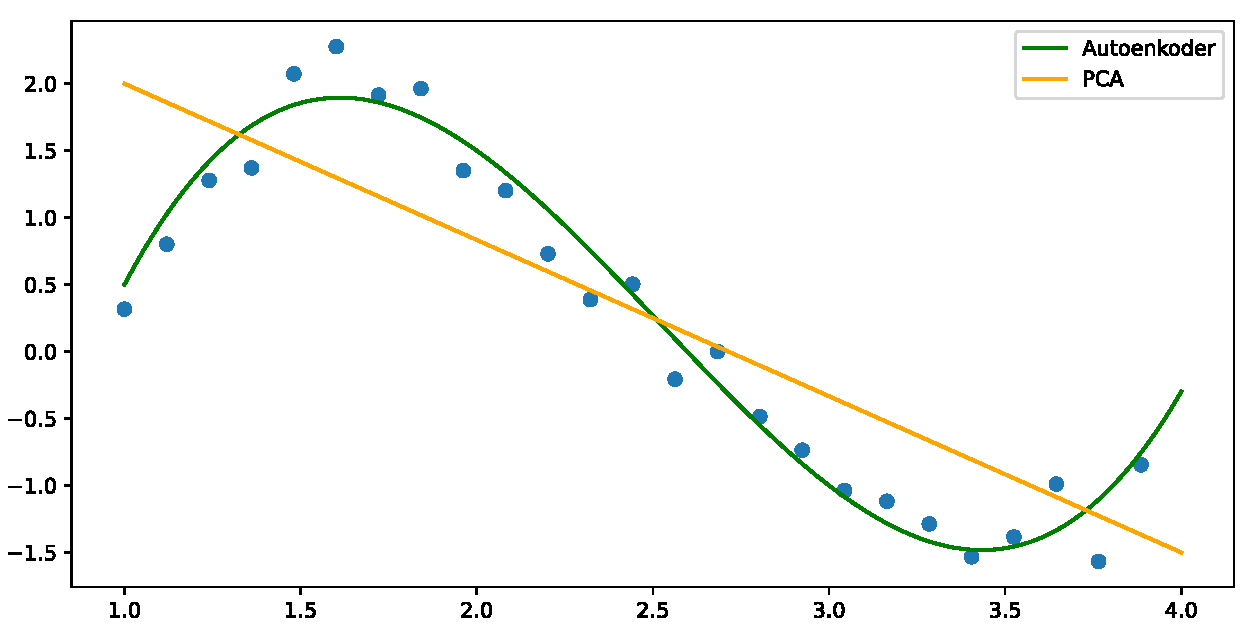
\includegraphics[width=14cm]{pcavsautoencoder.pdf}
	\label{fig:pcavsautoenkoder}
	\caption{Liniowe i nieliniowe przekształcenie.}
\end{figure}

\subsection{Odszumianie obrazów}
Model autoenkodera przeznaczony do odszumiania danych często dostaje swoją nazwę i jest określany mianem DAE \textit{(Denoising autoencoder)}. DAE, tak jak zwykły autoenkoder, próbuje w jak najlepszy sposób skompresować dane, zachowując jak najwięcej istotnych informacji. Najważniejszą różnicą między tymi modelami są dane, które dostają na wejście i wyjście. Obrazy przyjmowane na warstwę wejściową są zaszumione, natomiast te z warstwy wyjściowej pochodzą prosto ze zbioru danych.
Powodem, dla którego autoenkodery tak dobrze nadają się do odszumiania, jest ich umiejętność kompresji danych. Kompresja, której dokonują te modele jest stratna. W przypadku, kiedy naszym głównym zadaniem jest jak najlepsze odtworzenie danych wejściowych, jest to kłopot, jednak w tym przypadku możemy wykorzystać tę własność na naszą korzyść. Porównując wyjście modelu z danymi bez szumu, zapewniamy, że model nauczy się w jakimś stopniu odtwarzać je poprawnie. Zmuszamy w ten sposób model do ignorowania nieistotnych części naszych danych oraz zapamiętywanie tylko tych, na podstawie których będzie możliwe jak najlepsze odwzorowanie wejścia sieci.
Rysunek \ref{fig:noisedae} pokazuje możliwości modelu na przykładzie zbioru danych MNIST. Do obrazów przeznaczonych do treningu został dodany szum. Zaszumiony obraz powstał przez dodanie do oryginalnego obrazu losowo wybranych wartości z rozkładu Gaussa $\mathcal{N}(0,1)$ przemnożonych przez stałą, która w tym przypadku wynosi $0,4$. Następnie obrazy wejściowe zostały skompresowane do kodu o długości 5, a następnie odkodowane przez dekoder. 
\begin{figure}[h!]
	\centering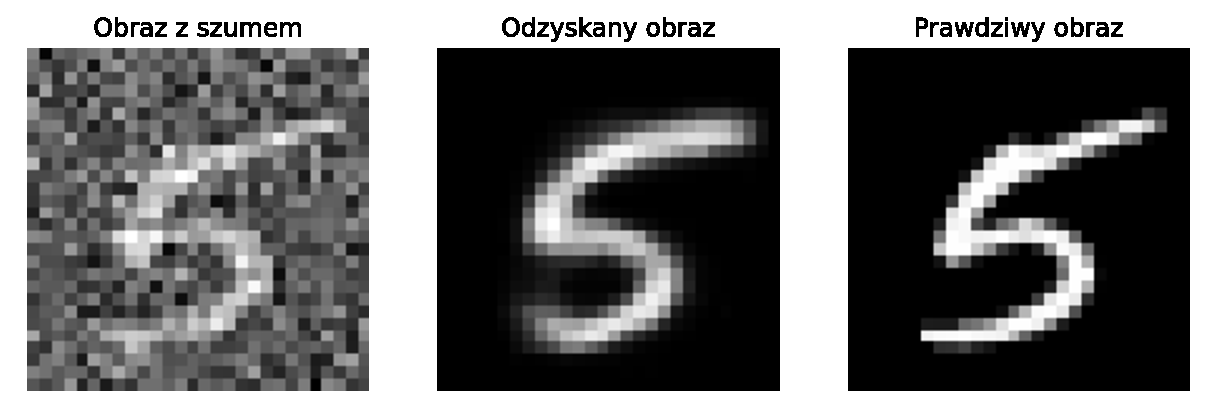
\includegraphics[width=14.5cm]{denoisingae.pdf}
	\caption{Obraz z szumem, odzyskany oraz prawdziwy.}
	\label{fig:noisedae}
\end{figure}

Wadą autoenkoderu przeznaczonego do odszumiania danych jest jego ścisłe powiązanie ze zbiorem danych, na których został wytrenowany. Model z parametrami wytrenowanymi na jednym zbiorze danych nie będzie się nadawał do innego zbioru, z którego danymi będziemy chcieli pracować. Jedynym rozwiązaniem tego problemu jest stworzenie nowego modelu przeznaczonego do użytku na nowych danych. 
\subsection{Uzupełnianie obrazów}
Uzupełnianie obrazów ma na celu wypełnienie brakującej lub zamaskowanej części obszaru. Człowiek jest w stanie sobie poradzić z tym zadaniem bez problemu, jednak dla komputera nie jest ono oczywiste. Bierze się to z tego, że jest ogromna ilość możliwości wypełnienia nawet niewielkiej brakującej przestrzeni. 
Można wyróżnić dwa główne podejścia wypełniania obrazów:
\begin{itemize}
	\item sieć posiada informację, w którym miejscu obrazu jest luka;
	\item sieć musi sama się nauczyć, które miejsce obrazu musi wypełnić.
\end{itemize}
Rysunek \ref{fig:lukaae} przedstawia drugie podejście. 
\begin{figure}[h]
	\centering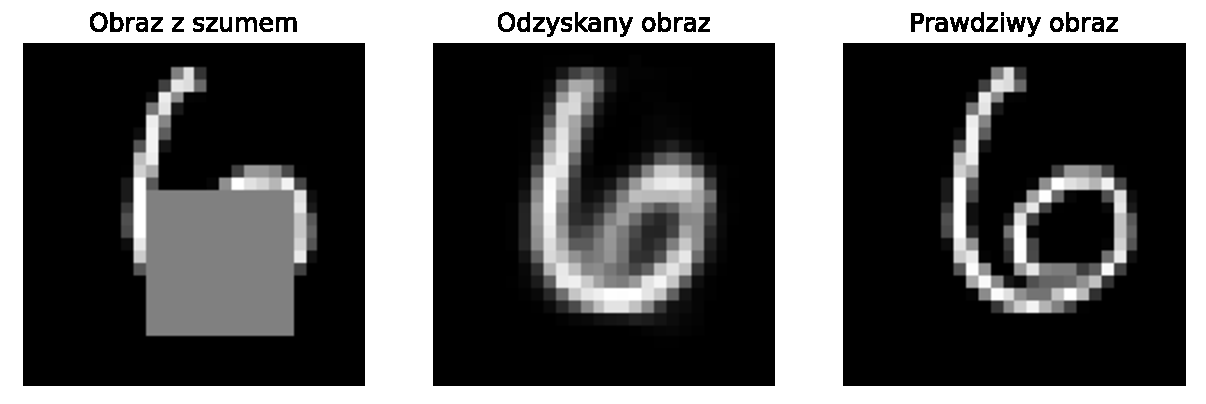
\includegraphics[width=14.5cm]{completionae.pdf}
	\caption{Obraz z luką, odzyskany oraz prawdziwy.}
	\label{fig:lukaae}
\end{figure}

\section{Problemy z generacją nowych danych}
Dobrym pytaniem jest, czy przy pomocy kodu jesteśmy generować nowe dane podobne do tych, na których model został wytrenowany. Wiemy, że sieć po treningu, jest w stanie ze zmiennych ukrytych odkodować obraz, więc ustawiając wejście dekodera na losowy punkt z przestrzeni zmiennych, powinniśmy być w stanie dostać obraz, który jest podobny do tych, na których sieć została wytrenowana.
Aby model mógł generować nowe dane, muszą zostać spełnione dwa warunki:
\begin{itemize}
	\item Nasza przestrzeń kodu (tzw. zmiennych ukrytych) musi być ciągła, co znaczy, że dwa punkty znajdujące się obok siebie będą dawać podobne dane kiedy zostaną odkodowane.
	\item Przestrzeń musi być kompletna, co znaczy, że punkty wzięte z dystrybucji muszą dawać wyniki mające sens.
\end{itemize}
Tradycyjna architektura nie zapewnia nam przed treningiem żadnego z tych warunków.
Spoglądając na rysunek \ref{fig:latentspaceae}, możemy zaobserwować, że przestrzeń zawiera luki. Szczególnie dobrze to widać między klasami oznaczającymi jedynki oraz siódemki. Kolejnym problemem widocznym na tej grafice jest brak separacji między klasami. Niektóre z nich są dobrze odseparowane od siebie, jednak inne całkowicie na siebie nachodzą, jak siódemki z dziewiątkami czy trójki z piątkami. Zadaniem modelu jest jak najlepsze odzwierciedlenie skompresowanych danych, a nie dbanie o to, czy rozkład zmiennych kodu spełnia nasze warunki. Może się tak zdarzyć, że sieć nauczy się akurat takiej dystrybucji, która nam pasuje, ale jest to bardzo mało prawdopodobne. Jeśli chcemy zbudować model generacyjny, musimy mieć zagwarantowane, że za każdym razem dostaniemy rozkład spełniający odpowiednie warunki. 
\chapter{Wariacyjny autoenkoder}
\section{Informacje ogóle}
Wariacyjny autoenkoder (VAE) rozwiązuje problemy generacyjne tradycyjnego modelu. VAE ma na celu skompresowanie danych do określonego wielowymiarowego rozkładu ukrytego, a następnie z próbki tej dystrybucji próbuje jak najlepiej zrekonstruować wejście. Model ten należy go grupy wariacyjnych metod Bayesowskich, czemu zawdzięcza swoją nazwę. Dystrybucjami najczęściej wybieranymi do reprezentacji zmiennych ukrytych są rozkłady normalne. Rozkład normalny jest opisywany przy pomocy dwóch wartości: średnia, która oznaczana jest znakiem $\mu$ oraz odchylenie standardowe oznaczane $\sigma$. Jeśli chcemy dane skompresować do kodu o długości $n$, enkoder wygeneruje dwa wektory $n$-wymiarowe, z którego jeden będzie przechowywał wartości średniej, a drugi odchylenia standardowego dla każdego z $n$ rozkładów normalnych co przedstawia rysunek \ref{fig:vaeschemat}.
\begin{figure}[h!]
	\centering
	\begin{tikzpicture}
		\node (true) at (-7, 0) {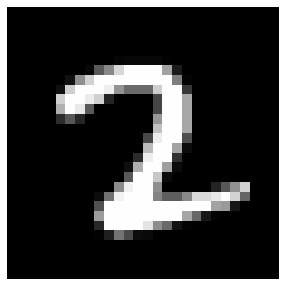
\includegraphics[width=2.5cm]{vaeorg1.png}};
		\draw[thick] (-4.8, 1) -- (-4.8, -1) node[pos=0.5] (enkoderin){} -- (-3.7, -0.6) -- (-3.7, 0.6) node[pos=0.5] (enkoderout){} -- cycle;
		\draw[-latex, thick] (true.east) -- (enkoderin.west);                                                                                 
		\node[scale=0.7](meanv) at (-2.5, 0) {\(\begin{bmatrix}                                                                                
		1.88 \\ 1.24 \\ \vdots \\ 2.09 \\ 2.18                                                                                        
		\end{bmatrix}\)};                                                                                                                     
		\node[scale=0.7] (stdv) at (-1.5, 0) {\(\begin{bmatrix}                                                                              
            0.34 \\ 0.92 \\ \vdots \\ 1.69 \\ 0.15                                                                        
			\end{bmatrix}\)};                                                                                                                    
		\draw[-latex, thick](enkoderout.east) -- (meanv.west);                                                                                 
		\node[scale=0.7] (nv) at (0.5, 0) {\(\begin{bmatrix}                                                                                  
				 \mathcal{N}(1.88,0.34)\\ \mathcal{N}(1.24,0.92) \\ \vdots \\ \mathcal{N}(2.09,1.69) \\ \mathcal{N}(2.18,0.15)
			\end{bmatrix}\)};
		\draw[-latex, thick] (stdv.east) -- (nv.west);
		\node[scale=0.7] (sample) at (2.5, 0) {\(\begin{bmatrix}
				1.28 \\ 1.87 \\ \vdots \\ 2.01 \\ 2.28
			\end{bmatrix}\)};
		\draw[-latex, thick] (nv.east) -- (sample.west);
				\draw[thick] (3.7, 0.6) -- (3.7, -0.6) node[pos=0.5] (dekoderin){} -- (4.8, -1) -- (4.8, 1) node[pos=0.5] (dekoderout){} -- cycle;
		\node (recon) at (7, 0) {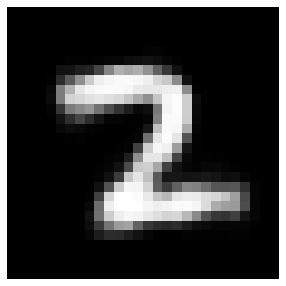
\includegraphics[width=2.5cm]{vaerec1.png}};
		\draw[-latex, thick](sample.east) -- (dekoderin.west);
		\draw[-latex, thick](dekoderout.east) -- (recon.west);
		% Labels
		\node at (-7, -1.5) {wejście};
		\node at (7, -1.5) {wyjście};
		\node at (-2.5, -1.5) {$\mu$};
		\node at (-1.5, -1.5) {$\sigma$};
		\node at (2.5, -1.5) {$z$};
		\node at (0.5, -1.5) {dystrybucje};
		\node at (-4.25, -1.5) {enkoder};
		\node at (4.25, -1.5) {dekoder};

	\end{tikzpicture}
	\caption{Schemat budowy wariacyjnego autoenkodera.}
	\label{fig:vaeschemat}
\end{figure}

 Ograniczając enkoder do nauki wyłącznie tej dystrybucji, z której losujemy zmienne ukryte, na podstawie których rekonstruujemy obrazy, zapewniamy sobie gładką oraz ciągłą dystrybucje zmiennych losowych. Dekoder patrząc na obraz wyjściowy i porównując go z prawdziwym, nauczy się odkodowywać niedaleko oddalone od siebie punkty z rozkładu w bardzo podobny sposób.

\begin{figure}[h!]
	\centering
	\pgfplotsset{
		colormap={whitered}{color(0cm)=(white); color(1cm)=(orange!75!red)}
	}
	\begin{tikzpicture}[
		declare function={mu1=2;},
		declare function={mu2=3;},
		declare function={sigma1=0.5;},
		declare function={sigma2=0.6;},
		declare function={normal(\m,\s)=1/(2*\s*sqrt(pi))*exp(-(x-\m)^2/(2*\s^2));},
		declare function={bivar(\ma,\sa,\mb,\sb)=
			1/(2*pi*\sa*\sb) * exp(-((x-\ma)^2/\sa^2 + (y-\mb)^2/\sb^2))/2;}]
		\begin{axis}[
			colormap name=whitered,
			width=15cm,
			view={45}{55},
			enlargelimits=false,
			grid=major,
			domain=0:5,
			y domain=0:5,
			samples=31,
			xlabel=$x_2$,
			ylabel=$x_1$,
			zlabel={$P$},
			]
			\addplot3 [surf] {bivar(mu1,sigma1,mu2,sigma2)};
			\addplot3 [domain=0:5,samples=31, samples y=0, thick, smooth] (x,5,{normal(mu1,sigma1)});
			\addplot3 [domain=0:5,samples=31, samples y=0, thick, smooth] (0,x,{normal(mu2,sigma2)});
			
			\draw [black!50] (axis cs:-1,0,0) -- (axis cs:4,0,0);
			\draw [black!50] (axis cs:0,-1,0) -- (axis cs:0,4,0);
			
			\node at (axis cs:0,2,0.12) [pin=165:$P(x_1)$] {};
			\node at (axis cs:4,4,0.32) [pin=-15:$P(x_2)$] {};
		\end{axis}
	\end{tikzpicture}
	\caption{Wielowymiarowy rozkład zmiennej.}
\end{figure}
\begin{figure}[h!]
	\centering
	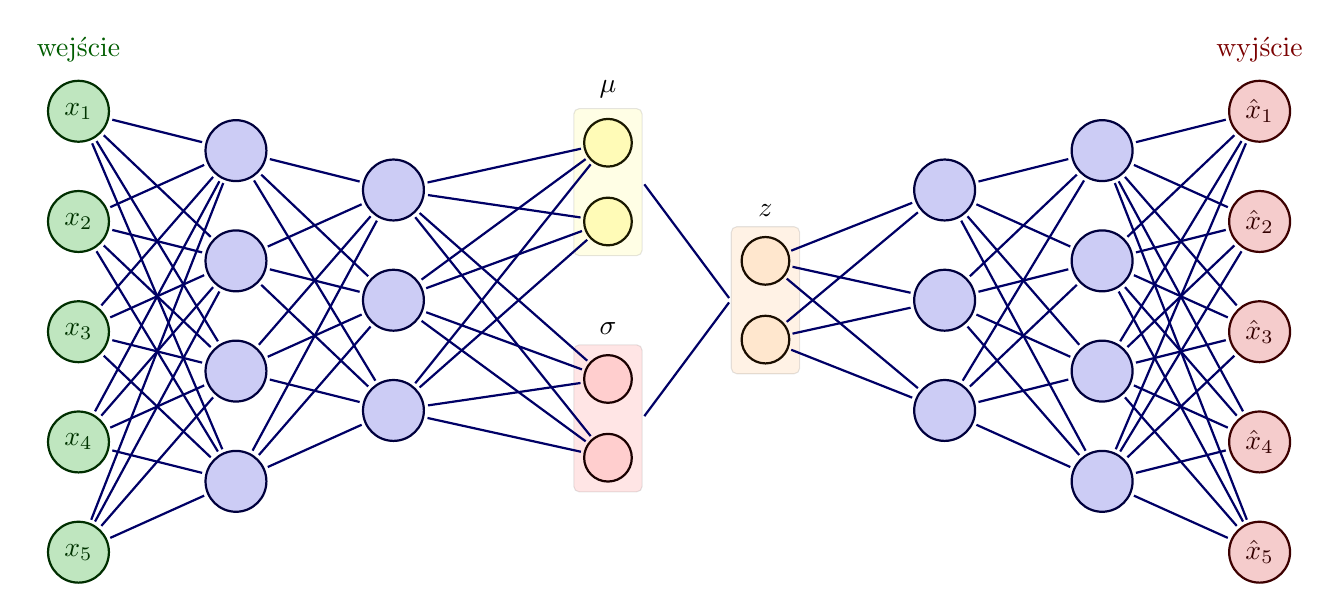
\begin{tikzpicture}[
		shorten >=1pt, shorten <=1pt,
		neuron/.style={circle, draw, minimum size=4ex, thick},
		hidden/.style={node,blue!20!black,draw=myblue!30!black,fill=myblue!20},
		myin/.style={node,green!20!black,draw=mygreen!30!black,fill=mygreen!25},
		myout/.style={node,red!20!black,draw=myred!30!black,fill=myred!20},
		legend/.style={font=\large\bfseries},
		]
		
		% encoder
		\drawEncoder{encoder}{{{,,,,}, {,,,}, {,,}}}
		\denselyConnectNodes{encoder}{{5, 4, 3}}
		
		% decoder
		\begin{scope}[xshift=11cm]
			\drawDecoder{decoder}{{{,,}, {,,,}, {,,,,}}}
			\denselyConnectNodes{decoder}{{3, 4, 5}}
		\end{scope}
		
		% mu, sigma, sample nodes
		\foreach \idx in {1,...,2} {
			\coordinate[neuron, right=2 of encoder-3-2, yshift=\idx cm, fill=yellow, fill opacity=0.2] (mu-\idx);
			\coordinate[neuron, right=2 of encoder-3-2, yshift=-\idx cm, fill=red, fill opacity=0.1] (sigma-\idx);
			\coordinate[neuron, right=4 of encoder-3-2, yshift=\idx cm-1.5cm, fill=orange, fill opacity=0.1] (sample-\idx);
		}
		
		% mu, sigma, sample boxes
		\node [label=$\mu$, fit=(mu-1) (mu-2), draw, fill=yellow, opacity=0.1, rounded corners=2] (mu) {};
		\node [label=$\sigma$, fit=(sigma-1) (sigma-2), draw, fill=red, opacity=0.1, rounded corners=2] (sigma) {};
		\node [label=$z$, fit=(sample-1) (sample-2), draw, fill=orange, opacity=0.1, rounded corners=2] (sample) {};
		
		% mu, sigma, sample connections
		\draw[connect] (mu.east) edge (sample.west) (sigma.east) -- (sample.west);
		\foreach \a in {1,2,3}
		\foreach \b in {1,2} {
			\draw[connect] (encoder-3-\a) -- (mu-\b);
			\draw[connect] (encoder-3-\a) -- (sigma-\b);
			\draw[connect] (sample-\b) -- (decoder-1-\a);
		}
		
		\node[above=0.1 of encoder-1-1,mygreen!60!black] {wejście};
		\node[above=0.1 of decoder-3-1,myred!60!black] {wyjście};
		
	\end{tikzpicture}
	\caption{Sieć neuronowa budująca model VAE.}
	\label{fig:vaenetwork}
\end{figure}

Sieć neuronowa budująca wariacyjny autoenkoder posiada dość nietypową budowę. Ostatnia ukryta warstwa enkodera łączy się z dwiema niepołączonymi ze sobą warstwami reprezentującymi średnią oraz odchylenie standardowe normalnej dystrybucji, której chcemy się nauczyć. Obie warstwy łączą się w jedną, która dokonuje operacji próbkowania z dystrybucji na nauczonych parametrach. Warstwy reprezentujące średnią, odchylenie standardowe oraz zmienne ukryte muszą posiadać taką samą liczbę neuronów, przedstawiającą długość wektora reprezentującego skompresowane dane.
\section{Formuła matematyczna}
Model VAE mimo swojego podobieństwa do tradycyjnego autoenkodera znacznie różni się w formulacji matematycznej. Największe różnice obserwujemy w zachowaniu enkodera. Kod, który on produkuje, nazywamy wartościami ukrytymi, ponieważ musimy go wywnioskować na podstawie każdej danej. Trenując tradycyjny model, nie patrzymy na to, co wiemy o dystrybucji $p(z|x)$, z której pochodzą zmienne. Enkoder wariacyjnego autoenkodera jest, jak już zostało powiedziane, zobowiązany do nauki dystrybucji naszego wyboru. Wyrażenie $p(z|x)$ rozumiemy jako dystrybucję generującą zmienne ukryte na podstawie przedstawionej danej $x$. Chcemy policzyć ten rozkład. Twierdzenie Bayesa mówi nam, że:
\begin{center}
	$p(z|x)=\dfrac{p(x|z)p(z)}{p(x)}$
\end{center}
Aby obliczyć rozkład marginalny $p(x)$, musimy policzyć:
\begin{center}
	$p(x) = \displaystyle\int_{z}^{}p(x|z)p(z)dz$
\end{center}
Obliczenie tej całki jest bardzo trudne lub nawet obliczeniowo niemożliwe w rozsądnym czasie, ponieważ $z$ jest często wielowymiarowym wektorem, a musimy całkować po wszystkich wymiarach. Aby próbować policzyć tę całkę w inny sposób, możemy wybrać jedną z dwóch metod:
\begin{itemize}
	\item próbkowanie Monte Carlo łańcuchami Markowa;
	\item wnioskowanie wariacyjne.
\end{itemize}
Przestrzeń przeszukiwań może być kombinatorycznie za duża, aby korzystać z pierwszej metody lub błąd przybliżenia tej całki będzie za duży w przypadku znacznej ilości wymiarów.
%\textit{citation needed :(} \\

\section{Wnioskowanie wariacyjne}
Wnioskowanie wariacyjne pozwala nam zastąpić jedną dystrybucje, o której nie wiemy za dużo i trudno z nią pracować na taką, jaka pasuje nam do problemu oraz dobrze odzwierciedla początkową. Używając tej metody, uda nam się rozwiązać problem policzenia rozkładu $p(z|x)$. Zastąpimy go rozkładem $q$, który będzie jak najlepiej odwzorowywał oryginalny rozkład. 
\begin{figure}[h!]
	\centering
	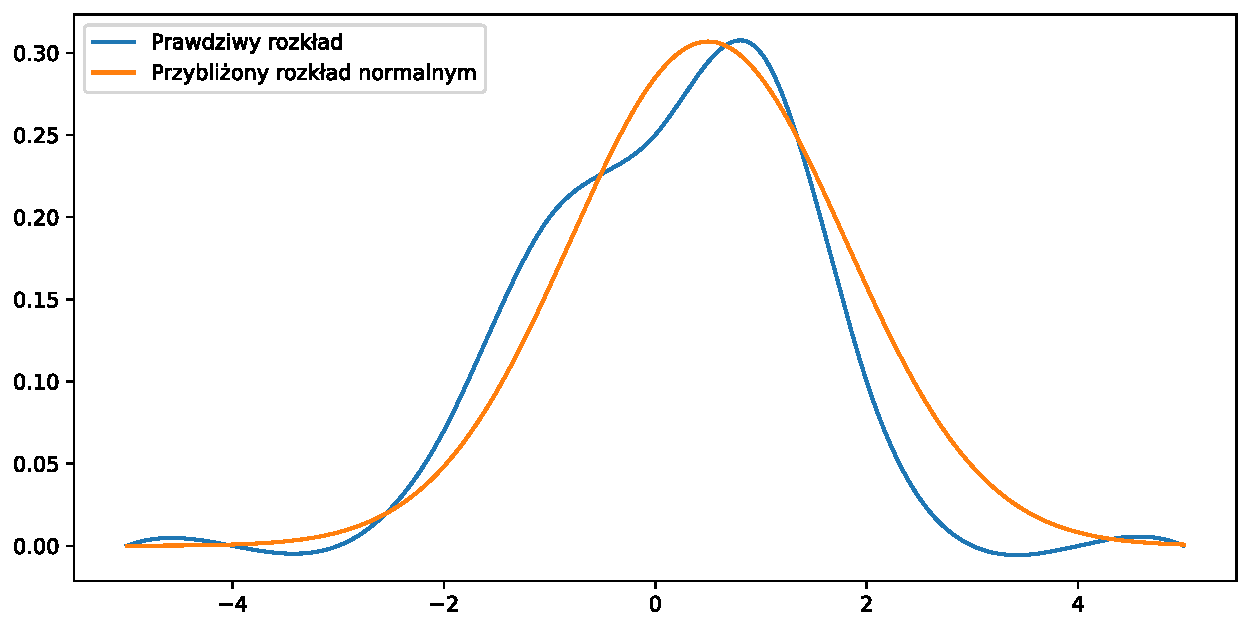
\includegraphics[width=12cm]{approximate.pdf}
	\label{fig:approximate}
	\caption{Prawdziwa oraz przybliżona dystrybucja.}
\end{figure} 

Wykres \ref{fig:approximate} przedstawia dwie krzywe. Pomarańczowa krzywa, opisująca rozkład normalny w bardzo dobry sposób, przybliża prawdziwą dystrybucję.
\subsection{Dywergencja Kullbacka-Leiblera}
Aby być w stanie zminimalizować błąd pomiędzy prawdziwą a zamienną dystrybucją, musimy posiadać miarę, która określi nam rozbieżność między dwoma rozkładami prawdopodobieństwa. Miarą tą jest dywergencja Kullbacka-Leiblera ($D_{KL}$). Podstawowymi jej własnościami są:
\begin{itemize}
	\item miary tej nie można określić mianem metryki, ponieważ nie jest symetryczna ($D_{KL}(P\|Q)\neq D_{KL}(Q\|P)$);
	\item jej wartość jest nieujemna; $D_{KL}(P\|Q)) \geq 0$. Miara przyjmuje wartość 0 tylko w przypadku kiedy $P$ i $Q$ są identycznymi dystrybucjami.
\end{itemize}
Naszym celem jest zminimalizowanie błędu, co sprawi, że rozkład $q(z|x)$ będzie jak najbardziej podobny do $p(z|x)$.
\begin{center}
	$q^\ast(z|x)=\operatorname*{argmin}_{q(z|x)\in Q}(D_{KL}(q(z|x)\|p(z|x)))$
	\\gdzie $Q$ to rodzina prostych dystrybucji, na przykład rozkładu Gaussa.
\end{center}
\subsection{Dolna granica dowodów}
Zapiszmy, że:
\begin{center}
%	$D_{KL}(q(z|x)\|p(z|x))=\mathbb{E}_{z\sim q(z|x)}\log\dfrac{p(z|x)}{q(z|x)} = 
%	\displaystyle\int_{z}^{}q(z|x)\log\frac{q(z|x)}{p(z|x)}dz$
	$D_{KL}(q(z|x)\|p(z|x))=\displaystyle\int_{z}^{}q(z|x)\log\frac{q(z|x)}{p(z|x)}dz$
\end{center}
Policzenie $q(z|x)$ jest proste, ponieważ sami dobieramy sobie, jaką dystrybucją jest $q$. W naszym przypadku jest to rozkład normalny. Mimo to, obliczenia nie są możliwe, ponieważ natrafiamy znowu na problem wyznaczenia $p(z|x)$. Tym razem możemy przepisać:
\begin{center}
	$p(z|x)=\dfrac{p(x,z)}{p(x)}$
\end{center}
Podstawmy teraz zapisaną inaczej wartość $p$ do wzoru na dywergencję.
\begin{center}
	$D_{KL}(q(z|x)\|p(z|x))=\displaystyle\int_{z}^{}q(z|x)\log\frac{q(z|x)}{p(x,z)}p(x)dz$
\end{center}
Własności logarytmów pozwalają nam zamienić iloczyn pod logarytmem na sumę w następujący sposób:
\begin{center}
	$D_{KL}(q(z|x)\|p(z|x))=\displaystyle\int_{z}^{}q(z|x)\left( \log\frac{q(z|x)}{p(x,z)} + \log p(x)\right) dz$
\end{center}
Mnożąc $q(z|x)$ przez nawias, otrzymujemy sumę pod całką, co możemy zapisać jako sumę dwóch całek. Następnie wartość $\log p(x)$ możemy wyłączyć przed całkę, ponieważ całkując po $z$, traktujemy ten logarytm jako stałą.
\begin{center}
	$D_{KL}(q(z|x)\|p(z|x))=\displaystyle\int_{z}^{}q(z|x)\left( \log\frac{q(z|x)}{p(x,z)}\right)dz + \log p(x)\underbrace{\displaystyle\int_{z}^{}q(z|x)dz}_{\text{$\alpha$}}$
\end{center}
Wartość całki zaznaczonej jako $\alpha$ jest równa 1, dlatego, że całkujemy funkcję dystrybucji prawdopodobieństwa po $z$, więc warunek dla $x$ nie ma dla nas znaczenia. Daje to nam:
\begin{center}
	$D_{KL}(q(z|x)\|p(z|x))=\underbrace{\displaystyle\int_{z}^{}q(z|x)\left( \log\frac{q(z|x)}{p(x,z)}\right)dz}_{\text{$\mathcal{L}$}} + \log p(x)$
\end{center}
Na razie nie dokonaliśmy żadnych obliczeń, tylko przepisaliśmy wzór na dywergencję.
\begin{center}
	$D_{KL}(q(z|x)\|p(z|x))= \mathcal{L} + \log p(x)$\\
	$-\mathcal{L} = \log p(x) - D_{KL}(q(z|x)\|p(z|x))$
\end{center}
Wartość $\log p(x)$ nosi nazwę dowodu, ponieważ mówi o prawdopodobieństwie otrzymania obserwacji $x$ przez nasz model.
Parametr $-\mathcal{L}$ nazywamy dolną granicą dowodu \textit{Evidence Lower BOund, \textbf{ELBO}}. Nazwa pochodzi od własności, mówiącej o tym, że jej wartość jest zawsze mniejsza lub równa dowodowi. Własność ta bierze się z faktu, że 
dywergencja jest zawsze nieujemna, a w naszym przypadku nawet dodatnia. 
\begin{center}
	$\mathcal{L}\leq\log p(x)$
\end{center}
Wartość dowodu jest stała dla podanego $z$, więc problem minimalizacji dywergencji możemy zapisać jako:
\begin{equation}
	\operatorname*{argmin}D_{KL}(q(z|x)\|p(z|x)) = \operatorname*{argmin}\mathcal{L} = \operatorname*{argmax}-\mathcal{L}
	\label{equ:argmindkl}
\end{equation}
\subsection{Funkcja straty}
Wiedząc z twierdzenia Bayesa, że $p(x,z) = p(x|z)p(z)$ możemy przepisać $\mathcal{L}$ jako:
\begin{center}
	$\mathcal{L}=\displaystyle\int_{z}^{}q(z|x)\left( \log\frac{q(z|x)}{p(x,z)}\right)dz=$\\
	$\displaystyle\int_{z}^{}q(z|x)\left( \log\frac{q(z|x)}{p(x|z)p(z)}\right)dz$
\end{center}
Korzystając kolejny raz z własności logarytmów, zapisujemy:
\begin{center}
	$\mathcal{L}=\displaystyle\int_{z}^{}q(z|x)\log\frac{q(z|x)}{p(z)}dz - \displaystyle\int_{z}^{}q(z|x)\log\frac{q(z|x)}{p(x|z)}dz$
\end{center}
Interpretując poszczególne składniki, dostajemy:
\begin{center}
	$\mathcal{L} =  D_{KL}(q(z|x)\|p(z)) - \mathbb{E}_{z\sim q(z|x)}\log p(x|z)$
\end{center}
Równanie \ref{equ:argmindkl} pokazuje, że minimalizacja pierwotnej dywergencji oznacza również minimalizację $\mathcal{L}$. 

Pierwsze wyrażenie reprezentuje odległość pomiędzy naszą dystrybucją zastępującą $p(z|x)$, czyli dystrybucją nauczona przez enkoder a $p(z)$, czyli rozkład zmiennych ukrytych, który jest przez nas wybierany. W naszym przypadku będzie to rozkład normalny. Drugie wyrażenie to wartość oczekiwana logarytmu prawdopodobieństwa otrzymania obserwacji $x$ z wartości ukrytych wybieranych z dystrybucji $q(z|x)$, której nauczył się enkoder.

Enkoder, jak i dekoder jesteśmy w stanie zapisać jako rozkłady prawdopodobieństwa. Funkcja $q(z|x)$ powie nam, jakie zmienne ukryte $z$ reprezentują daną $x$, natomiast $p(x|z)$ generuje nam dane na podstawie otrzymanego kodu. $q(z|x)$ jest dystrybucją enkodera, a $p(x|z)$ dekodera.

Wariacyjny autoenkoder poruszany w pracy generuje zmienne ukryte z rozkładu normalnego $p(z)=\mathcal{N}(0,\textit{\textbf{I}})$. Jeśli weźmiemy wszystkie nasze dane $x$ i przepuścimy je przez enkoder, wiemy, że próbkowane wartości przekazywane następnie do dekodera będą rozłożone normalnie. Rozwiązuje nam to problem tradycyjnego autoenkodera, którego zmienne ukryte są rozrzucone w sposób, który nie jesteśmy w stanie kontrolować. Znając już naszą dystrybucję, możemy policzyć dywergencję pomiędzy dwoma rozkładami normalnymi.
\begin{center}
	$\dfrac{1}{2}\displaystyle\sum_{D}^{i=1}\left\{\left(\dfrac{\sigma_0}{\sigma_1}\right)^2+\dfrac{(\mu_1 - \mu_0)^2}{\sigma_1^2} - 1 + 2\log\dfrac{\sigma_1}{\sigma_0}\right\}$
\end{center}
W naszym przypadku, gdzie $\mu_1 = 0$ oraz $\sigma_1=1$ uprości się do:
\begin{equation}
	\dfrac{1}{2}\displaystyle\sum_{D}^{i=1}\sigma_i^2+\mu_i^2-2\log(\sigma_i)-1
	\label{equ:kld_loss}
\end{equation} 
gdzie D to długość wektora zmiennych ukrytych. Jest to pierwsza część naszej funkcji straty. 

Druga część funkcji straty jest nazywana błędem rekonstrukcji. Możemy zastąpić wartość oczekiwaną wartością jednej próbki, ponieważ do trenowania wag modeli używamy metody gradientu stochastycznego. Aby uniknąć liczenia skomplikowanych dystrybucji prawdopodobieństwa $\log p(x|z)$, gdzie poszczególne wymiary $x$ są zależne od siebie, liczymy proste rozkłady na każdym wymiarze osobno. Aby to osiągnąć, używamy binarnej entropii krzyżowej. W praktyce często stosujemy również inne funkcje, takie jak błąd średnio-kwadratowy, będący bardziej intuicyjnym rozwiązaniem.
Możemy tak zrobić, ponieważ wartość prawdopodobieństwa należy do przedziału $\left[ 0, 1\right] $, więc ujemny logarytm z małej liczby (słabego odwzorowania wejścia przez dekoder) będzie ogromna liczbą, a z bliskiej jedynki -- małą. W ten sam sposób zachowuje się średni błąd kwadratowy.
\newpage
\subsection{Sztuczka reparametryzacyjna}
Model \textit{VAE} po zakodowaniu wejścia dokonuje operacji próbkowania (\textit{sampling}) z dystrybucji na nauczonych parametrach. Przy propagacji do przodu nie jest to problem, jednak podczas propagacji wstecznej jest to niemożliwe. Operacja próbkowania nie jest różniczkowalna, co sprawia, że nie możemy policzyć gradientu, po którym będziemy schodzić. Sposobem obejścia tego problemu jest zastosowanie sztuczki (\textit{reparameterization trick}). Próbkowanie z dystrybucji $z\sim\mathcal{N}(\mu, \sigma)$ jesteśmy w stanie zapisać jako:
\begin{center}
	$\epsilon\sim\mathcal{N}(0,1)$\\
	$z=\mu+\sigma\bigodot\epsilon$
\end{center} 
Pozornie nic się nie zmieniło, jednak teraz jesteśmy w stanie poprowadzić gradient przez $z$, które jest teraz deterministycznie. W poprzednim przypadku było ono losowe wybierane z dystrybucji. \\
\begin{figure}[h!]
	\centering
	\begin{tikzpicture}
		\node (dc) at (-4,0) {Dekoder};
		\node[shape=circle, draw=black, scale=1.2] (z) at (-4,-2) {$z$};
		\node (q) at (-2.6,-2) {$\sim q(z|x)$};
		\node[shape=diamond, draw=black] (sigma) at (-4,-4) {$\sigma$};
		\node[shape=diamond, draw=black] (mu) at (-6, -4) {$\mu$};
		\node (en) at (-5, -6) {Enkoder};
		
		\path[->] (z) edge node[left] {} (dc);
		\path[->] (mu) edge node[left] {} (z);
		\path[->] (sigma) edge node[left] {} (z);
		\draw[-to](-5, -5.5) -- (-5, -4.5);
		
		\node (dc1) at (4,0) {Dekoder};
		\node[shape=diamond, draw=black] (z1) at (4,-2) {$z$};
		\node (q1) at (6,-2) {$z=\mu+\sigma\bigodot\epsilon$};
		\node[shape=diamond, draw=black] (sigma1) at (4,-4) {$\sigma$};
		\node[shape=diamond, draw=black] (mu1) at (2, -4) {$\mu$};
		\node (en1) at (3, -6) {Enkoder};
		\node[shape=circle, draw=black, scale=1.2] (epsilon) at (6, -4) {$\epsilon$};
		\node (n) at (7.5, -4) {$\sim\mathcal{N}(0,1)$};
		
		\path[->] (z1) edge node[left] {} (dc1);
		\path[->] (mu1) edge node[left] {} (z1);
		\path[->] (sigma1) edge node[left] {} (z1);
		\path[->] (epsilon) edge node[left] {} (z1);
		\draw[-to](3, -5.5) -- (3, -4.5);
		
		\draw[-to](-1.5, -2) -- (2, -2) node[midway, above]{Reparametryzacja};
		
		\node[shape=diamond, draw=black, scale=1.2] (legend-diamond) at (-6, -7) {};
		\node[shape=circle, draw=black, scale=1.4] (legend-circle) at (-6, -8) {}; 
		\node (determin) at (-3, -7) {- węzeł deterministyczny};
		\node (randnode) at (-3.94, -8) {- węzeł losowy};
	\end{tikzpicture}
	\caption{Graficzna reprezentacja reparametryzacji.}
\end{figure}
\section{Zastosowania}
Wariacyjny autoenkoder jako pochodna tradycyjnego modelu może zostać zastosowany do takich samych zadań, jak detekcja anomalii, odszumianie oraz kompresja danych. Głównym jednak powodem, dla którego chcemy używać modelu VAE jest jego możliwość generowania danych. Mamy już znaną dystrybucję, z której możemy próbkować zmienne ukryte, aby generować nowe dane, podobne do oryginalnych ze zbioru danych. Rysunek \ref{fig:vaelatent} przestawia zmienne ukryte wygenerowane przez enkoder dla obrazków z MNIST. Porównując obrazek \ref{fig:vaelatent} z \ref{fig:latentspaceae} jasno widzimy, że model VAE rozwiązał omówione problemy generacyjne tradycyjnego autoenkodera. Przestrzeń jest kompletna i ciągła. Punkty dystrybucji znajdujące się blisko siebie generują podobne wyniki, co widać na obrazku \ref{fig:vaelatentgen}. Tak jak chcieliśmy, zmienne ukryte są rozłożone względem rozkładu normalnego. 

\begin{figure}[h!]
	\centering
	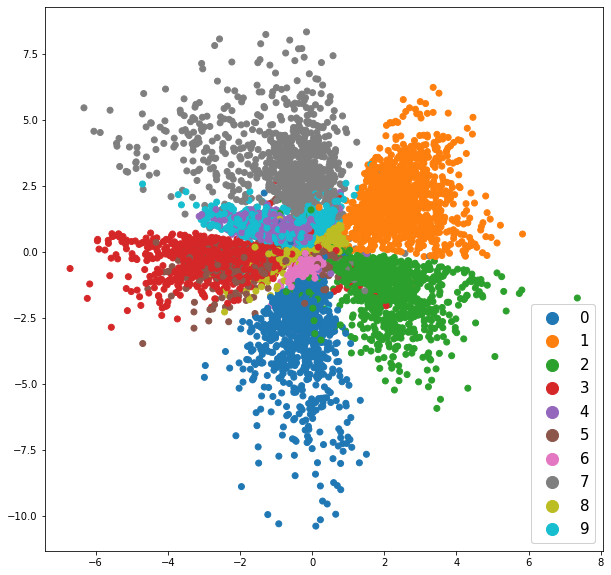
\includegraphics[width=14cm]{vaelatentspace.png}
	\caption{Przestrzeń zakodowanych zmiennych modelem VAE.}
	\label{fig:vaelatent}
\end{figure}
Obrazek \ref{fig:vaegeneracja} po lewej stronie pokazuje przykładowe dane ze zbioru danych MNIST, a prawa strona pokazuje dane wygenerowane przez wytrenowany model. Generując dane, nie potrzebujemy już enkodera. Na wejście dekoder dostaje losowo wybrane punkty z dystrybucji, którą wybraliśmy sobie podczas budowy modelu. W naszym przypadku jest to rozkład normalny.
\begin{figure}[h!]
	\centering
	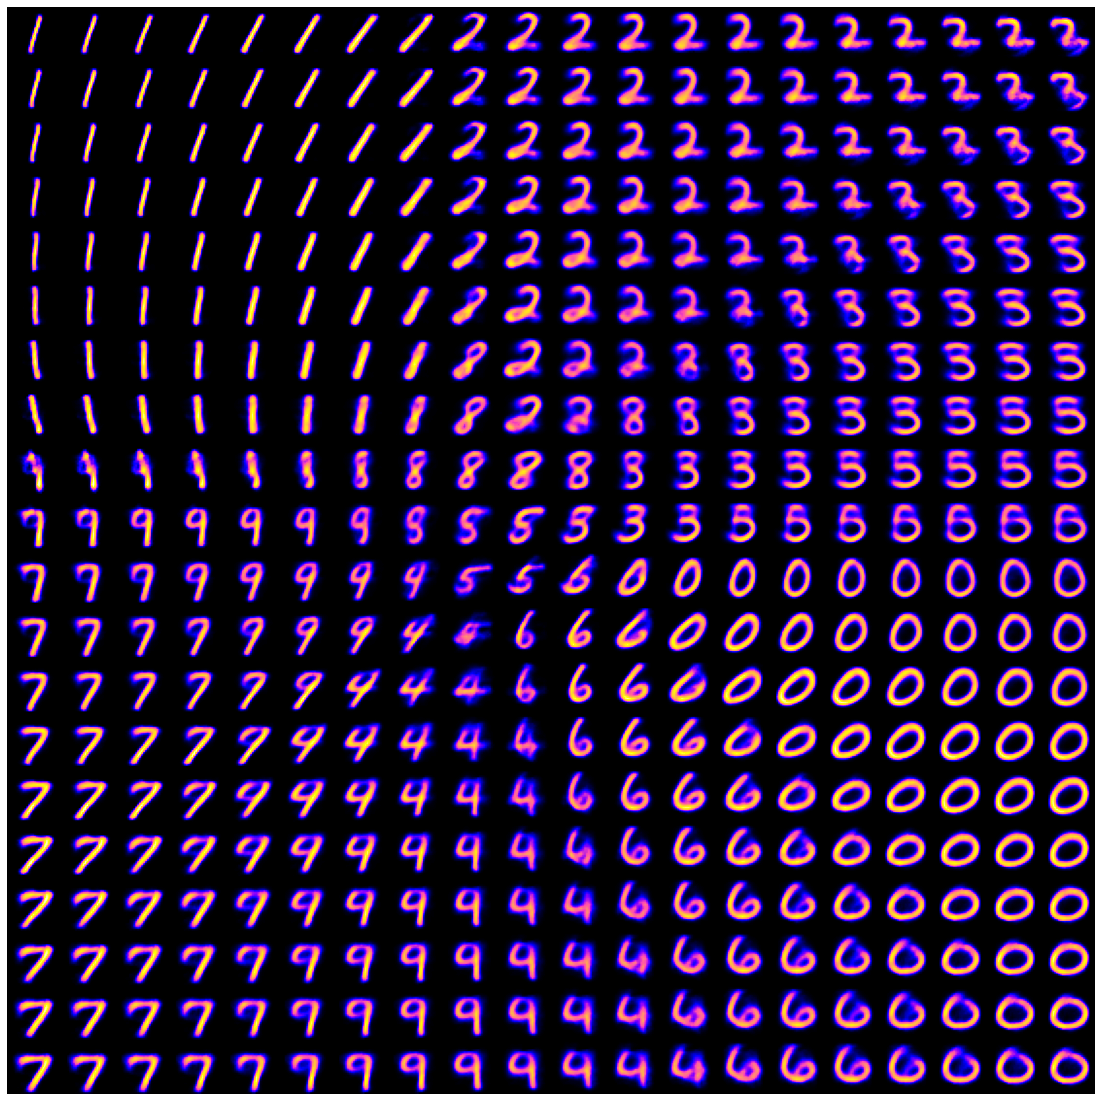
\includegraphics[width=14cm]{vaelatentgen.png}
	\caption{Wygenerowane obrazy modelem VAE na przestrzeni zmiennych.}
	\label{fig:vaelatentgen}
\end{figure}

\begin{figure}[h!]
	\centering
	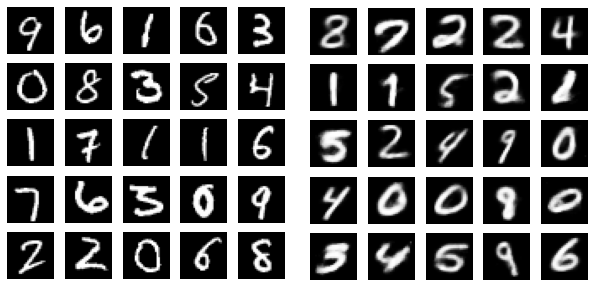
\includegraphics[width=12cm]{vaegeneracja.png}
	\caption{Porównanie prawdziwych oraz wygenerowanych obrazów.}
	\label{fig:vaegeneracja}
\end{figure}


\chapter{Implementacja}
\section{TensorFlow oraz Keras}
\subsection{Informacje ogóle}
TensorFlow jest jedną z najbardziej popularnych bibliotek implementującą metody uczenia maszynowego. Twórcą projektu jest Google, które udostępniło je jako wolne oprogramowanie. Biblioteka jest dostępna dla wielu języków programowania, jednak najczęściej jest używana, programując w języku Python. Programowanie bezpośrednio w TensorFlow jest dość skomplikowane, a kod jest mało czytelny. Problemy te rozwiązuje Keras, który jest nakładką na bibliotekę. 

Keras również jest darmową i otwartą biblioteką, jednak jest tylko przeznaczona dla języka Python. Implementuje prosty i przejrzysty sposób tworzenia modeli oraz sieci neuronowych. Poza tradycyjnymi, głębokimi architekturami możliwe jest tworzenie sieci rekurencyjnych oraz konwolucyjnych. Obie biblioteki wspierają rozproszone obliczenia na kartach graficznych. 

W implementacji modeli AE i VAE, użyteczną biblioteką będzie NumPy. Jest to wolnych projekt, umożliwiający operacje na macierzach oraz wektorach. Jako biblioteka napisana w języku C, dokonuje o wiele szybszych operacji w porównaniu do tych, które wykonywane by były w czystym Pythonie. 

Istnieje kilka możliwości implementacji tradycyjnego oraz wariacyjnego autoenkodera używając sieci gęstych, konwolucyjnych lub nawet rekurencyjnych takich jak LSTM (\textit{long short-term memory}). Każda z nich może nadać się do innych zbiorów danych, jednak wszystkie w kluczowych punktach działają w ten sam sposób. Wejście zostaje skompresowane do odpowiedniej długości kodu, a w przypadku autoenkoderów wariacyjnych do wielowymiarowego rozkładu normalnego. 
\subsection{Implementacja w języku Python}
Importujemy potrzebne klasy do implementacji obu modeli.
\begin{figure}[h!]
	\centering
	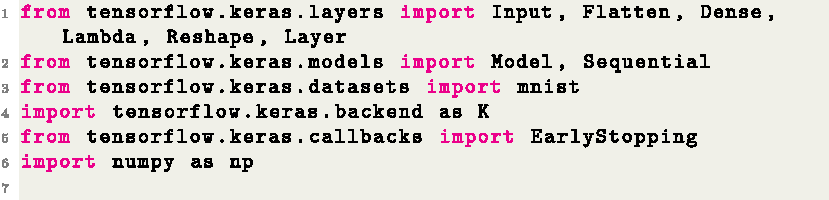
\includegraphics[width=\linewidth]{importy.pdf}
\end{figure}

Następnie wczytujemy zbiór danych MNIST, który podzielony jest na część przeznaczoną do treningu oraz do testów. Implementując modele, nie będziemy korzystać z oznaczeń, do jakiej klasy należą poszczególne dane, ponieważ oba modele na swoją warstwę wejściową, jak i wyjściową dostają te same obrazy. Aby nie było problemów z typem danych, zamieniamy wszystkie próbki na macierze, które przechowują dane w formacie float o długości 32 bitów. Następnie dane skalujemy do przedziału [0, 1], dzieląc każdy piksel każdego obrazka przez 255. Wiemy, że dane składają się z obrazów w skali szarości i każdy piksel opisuje liczba z przedziału [0, 255], więc zwykłe dzielenie może zastąpić inne rozwiązania skalowania danych. Wyciągamy sobie również wysokość i szerokość obrazów.
\begin{figure}[h!]
	\centering
	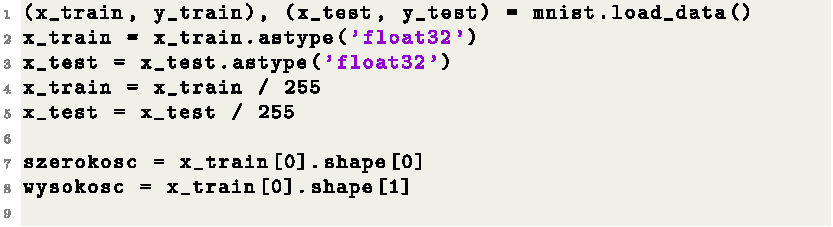
\includegraphics[width=\linewidth]{dane.pdf}
\end{figure}
\subsubsection{Autoenkoder}
Tworząc model, musimy zagwarantować odpowiednią architekturę. W tym przypadku używamy enkodera z dwiema warstwami ukrytymi, z czego pierwsza posiada 500 neuronów, a druga 120. Obraz jest kompresowany do kodu o długości 2. Architektura dekodera jest odbiciem lustrzanym enkodera. Funkcje aktywacji warstw ukrytych to ReLU \textit{Rectified Linear Unit}, które nie dość, że umożliwiają lepszą naukę sieci, to sprawiają, że trening zajmuje mniej czasu \cite{relu}. Używamy funkcji liniowej w warstwie kodu, aby nie ograniczać wartości, jakie poszczególne jego elementu mogą przyjąć. Funkcja sigmoidalna na wyjściu spłaszcza wyjście neuronu do przedziału [0, 1], czyli takiego samego, w jakim występują nasze dane.\\

Pierwsza warstwa wejściowa jest przeznaczona, aby przyjmować dane o wymiarze takim jak nasze obrazy. Następnie warstwa \textit{Flatten} zamienia dwuwymiarowe wejście na jednowymiarowe. Kolejne warstwy łączą się w normalny sposób pomiędzy sobą. Ostatnia warstwa \textit{Reshape} dokonuje odwrotnej operacji co \textit{Flatten}, zamieniając jednowymiarowe wartości na macierz, która ma takie same wymiary co dane wejściowe, co umożliwia porównanie wyniku modelu do wejścia. Tworzymy cały autoenkoder, używając klasy \textit{Model}, podając pierwszą oraz ostatnią warstwę. W ten sposób wszystkie parametry są trenowane na raz. Stworzenie osobno enkodera nie jest problemem, ponieważ posiada on tą samą warstwę wejściową co cały model. Dekoder jest nieco problematyczny, ponieważ musimy stworzyć jego własną warstwę wejściową, a następnie połączyć z nią warstwy modelu, tak aby korzystał z wytrenowanych parametrów. 
\begin{figure}[h!]
	\centering
	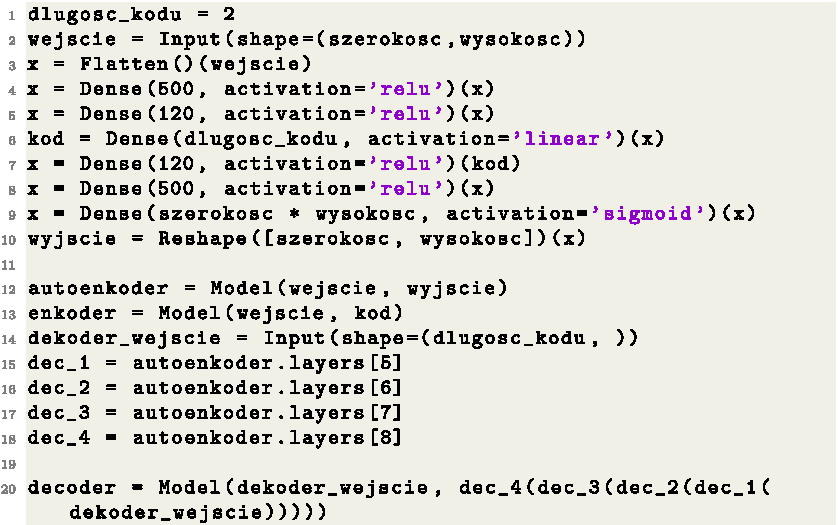
\includegraphics[width=\linewidth]{modelae.pdf}
\end{figure}

Zanim zaczniemy trenować naszą sieć, musimy sprecyzować funkcję straty oraz optymalizator. Funkcja użyta w tym przykładzie to błąd średnio-kwadratowy, który jest dobrym wyborem w przypadku porównywania obrazów. Optymalizator to algorytm znajdowania wag sieci, dla których funkcja straty jest jak najmniejsza, a co za tym idzie nasz model działa jak najlepiej. Wybraną metodą jest algorytm \textit{adam}, który jest pochodną stochastycznego gradientu. Obliczenia okupują mniej pamięci, jest prosty obliczeniowo oraz znajduje optymalne rozwiązanie szybciej niż tradycyjne podejście \cite{adam}. Jednym z jej twórców jest Diedrik Kingma, który również jako pierwszy zaproponował model wariacyjnego autoenkodera. Aby nie przetrenować modelu, dodajemy zbiór walidacyjny, który przejmuje 20\% danych treningowych. Walidacja służy nam do sprawdzenia na innych danych niż testowe i treningowe, czy model się nie przetrenował. W momencie, kiedy błąd na zbiorze walidacyjnym będzie rosnąć przez 3 epoki zamiast maleć, callback \textit{EarlyStopping} przerwie trening wag i przywróci wagi, dla których wynik był najlepszy.
\begin{figure}[h!]
	\centering
	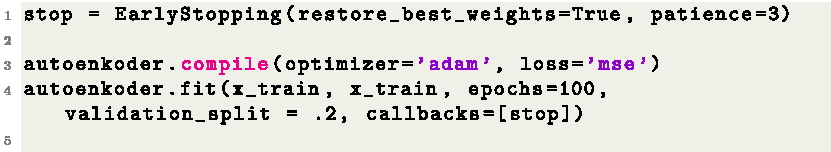
\includegraphics[width=\linewidth]{trainae.pdf}
\end{figure}

Po treningu modele są już gotowe go użytkowania. Aby dokonać przy ich pomocy obliczeń, wykonujemy funkcję \textit{predict}, do której podajemy odpowiednich wymiarów macierz. 
\subsubsection{Wariacyjny autoenkoder}
Przygotowanie zbioru danych dla wariacyjnego autoenkodera nie różni się w żaden sposób od pokazanego wyżej. 

Implementacja modelu VAE jest nieco bardziej skomplikowana niż AE. Bierze się to jego budowy, która wymaga rozłączenia jednej warstwy na dwie niezależne przyłączone do tej samej, co widać na obrazku \ref{fig:vaenetwork} oraz implementacji własnej funkcji straty. Warstwy reprezentujące średnią i odchylenie standardowe są połączone z ostatnią warstwą ukrytą. W naszym przypadku traktujemy jedną warstwę jako logarytm z odchylenia standardowego, ponieważ jego wartość nie może być ujemna. Kiedy chcemy użyć zmiennych, wystarczy, że dokonamy na nich operacji \textit{exp}. Funkcja \textit{probka} dokonuje losowania z dystrybucji na nauczonych parametrach, stosując opisaną wcześniej sztuczkę reparametryzacyjną. Zmienna \textit{eps} przechowuje wartości losowane z rozkładu normalnego i ich rozmiar jest równy ilości zmiennych ukrytych i wielkości partii danych (\textit{batch size}). Na etapie tworzenia architektury modelu jeszcze nie znamy wielkości batch-a, więc używając metody \textit{shape} będziemy ją dynamicznie zmieniać w zależności od przekazanych parametrów. Dostępna w paczce Keras warstwa \textit{Lambda} pozwala nam wywołać wskazaną funkcję na wartościach neuronów. Warstwę łączymy z obiema wcześniejszymi warstwami na raz. Implementacja dekodera jest identyczna jak dla tradycyjnego autoenkodera. Funkcja straty modelu VAE nie jest możliwa do automatycznego policzenia, tak jak zostało to pokazane w AE. Zmienna \textit{z$\_$odkodowane} będzie przechowywać obraz odkodowany ze zmiennych ukrytych, który będzie porównywany z tym przekazanym na wejście sieci.

\begin{figure}[h!]
	\centering
	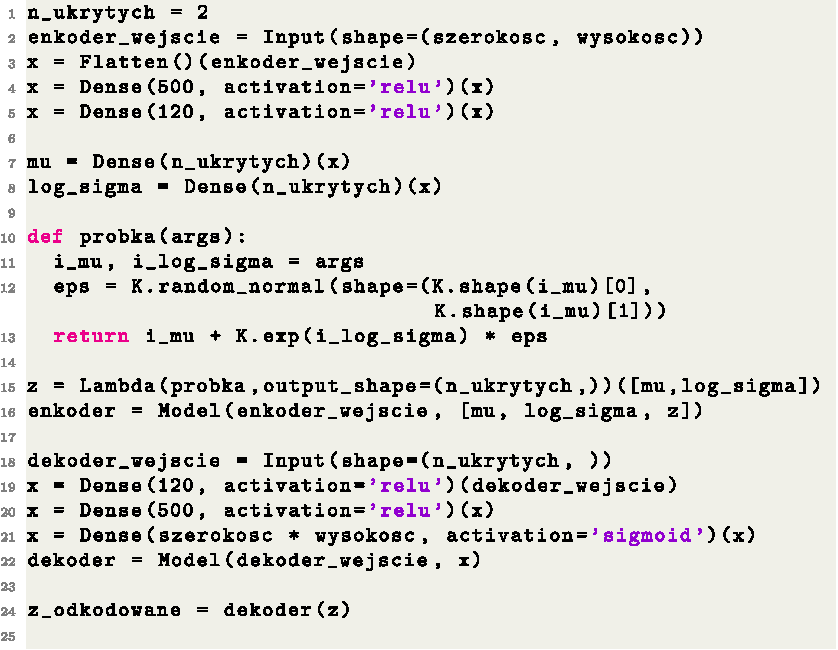
\includegraphics[width=\linewidth]{modelvae.pdf}
\end{figure}

\begin{figure}[h!]
	\centering
	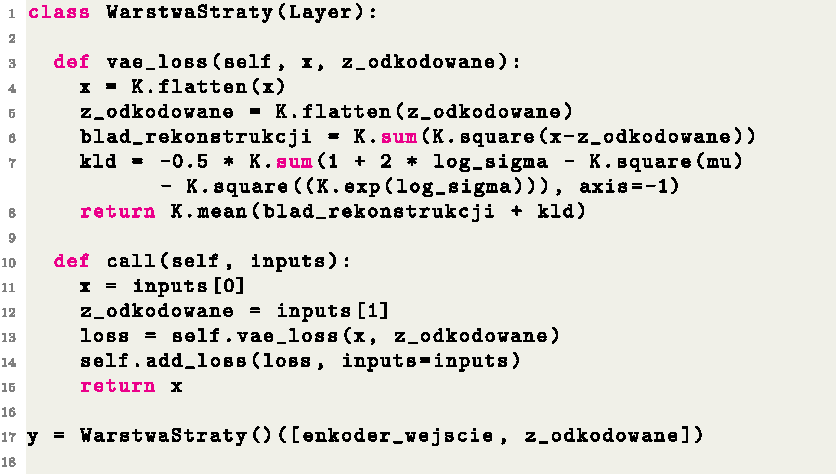
\includegraphics[width=\linewidth]{vaeloss.pdf}
\end{figure}

\newpage
Aby policzyć wartość funkcji straty, tworzymy nową warstwę przyłączoną do ostatniej. Jej jedynym zadaniem jest policzenie straty i nie ma ona możliwych do trenowania parametrów. Pierwsza funkcja oblicza wartość funkcji, a druga pozwala jej policzenie i minimalizacje przez model. Aby móc porównać obrazy, muszą być one w takich samych wymiarach, co gwarantujemy przez wywołanie funkcji \textit{flatten} na prawdziwym i odkodowanym obrazie. Błąd rekonstrukcji wybrany w tym przykładzie to błąd średnio-kwadratowy. Zmienna \textit{kld} przechowuje obliczoną wartość dywergencji Kullbacka-Leiblera z wyprowadzonego wzoru \ref{equ:kld_loss}. Warstwa obliczająca stratę jest połączona z wejściem i wyjściem całego modelu, co umożliwia dostęp do wejścia ze zbioru danych oraz obrazów odkodowanych ze zmiennych ukrytych. 


Posiadając warstwę obliczającą funkcję straty, możemy stworzyć model. Podczas kompilacji nie podajemy parametru \textit{loss}, ponieważ został on już dodany w naszej niestandardowej warstwie. Z tego samego powodu w funkcji mającej dokonać treningu modelu nie przekazujemy danych, do których jest porównywany wynik autoenkodera.
\begin{figure}[h!]
	\centering
	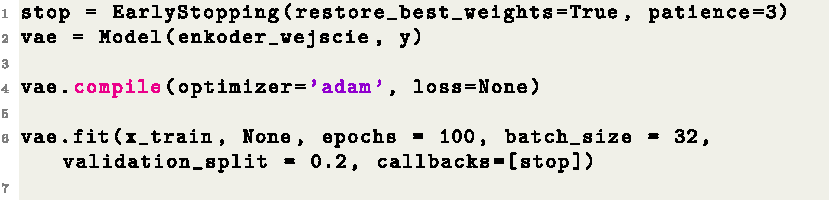
\includegraphics[width=\linewidth]{vaetrain.pdf}
\end{figure}

\chapter{Podsumowanie}
Autoenkoder tradycyjny oraz wariacyjny są podobnymi modelami uczenia maszynowego. Składają się z dwóch części: enkodera próbującego zakodować zmienne do kodu o określonej długości oraz dekodera rekonstruującego kod do danych wejścia sieci. Wariacyjny autoenkoder, zamiast generować zmienne bezpośrednio, wybiera je z wielowymiarowego rozkładu normalnego na nauczonych parametrach. Jest to sposób na rozwiązanie problemów z generacją nowych danych tradycyjnego modelu. Oba modele posiadają szerokie zastosowanie w kompresji oraz odszumianiu danych i detekcji anomalii. Przewaga wariacyjnego autoenkodera polega na jego umiejętności generacji danych, podobnych do tych, na których on został wytrenowany. 

%\listoftables{} % jeśli są tabele
%\addcontentsline{toc}{chapter}{Spis tabel}

\listoffigures{} % jeśli są tabele
\addcontentsline{toc}{chapter}{Spis rysunków}

\bibliographystyle{ieeetr}
\bibliography{./cytowania/cytowania.bib}
\end{document}
